% !TEX root =  fission.tex
%
% Use 'make' to run latex and generate the pdf file
%
% Doug Wright
%
% ADC 
%
% COK-2001-600 
% 11-304 Physics concepts such as hydrodynamics, photon transport,
% neutronics, fission, fusion, etc., when no classified information
% or association is revealed.

\documentclass[fleqn,11pt]{article}
\usepackage{h4}
\usepackage{url}
\usepackage{hyperref}  
	\hypersetup{linktocpage}	% only link the page number, too ugly if you highlight the text in the TOC
	\hypersetup{colorlinks}     % use color instead of box around link
	\hypersetup{linkcolor=blue} % use blue instead of default red, because it looks better
	\hypersetup{citecolor=blue}  	% default green does not show when printed, so use blue
\input{local}	% macro definitions for this document


\newcommand{\notgeant}[1]{#1} % include stuff that is not for geant manual

\date{October 17, 2016}

\version{}   % doc version number
\ucrl{UCRL-AR-}

\mytitle{Simulation of Neutron and Gamma Ray Emission\\ from Fission and Photofission}

\author{
J\'er\^ome M. Verbeke, Chris Hagmann, Doug Wright\footnote{
Contact info: wright20@llnl.gov, 925-423-2347}\\
\\
Lawrence Livermore National Laboratory
}

\begin{document}
\maketitle

\tableofcontents
\clearpage


\newpage \section*{Copyright notice}
Copyright (c) 2006-2016 Lawrence Livermore National Security, LLC.\\
Produced at the Lawrence Livermore National Laboratory \\
UCRL-CODE-224807.

All rights reserved. Redistribution and use in source and binary forms, with or without modification, are permitted provided that the following conditions are met:

\begin{itemize}
\item  Redistributions of source code must retain the above copyright notice, this list of conditions and the disclaimer below.

\item  Redistributions in binary form must reproduce the above copyright notice, this list of conditions and the disclaimer (as noted below) in the documentation and/or other materials provided with the distribution.

\item  Neither the name of the LLNS/LLNL nor the names of its contributors may be used to endorse or promote products derived from this software without specific prior written permission.
\end{itemize}

THIS SOFTWARE IS PROVIDED BY THE COPYRIGHT HOLDERS AND CONTRIBUTORS "AS IS" AND ANY EXPRESS OR IMPLIED WARRANTIES, INCLUDING, BUT NOT LIMITED TO, THE IMPLIED WARRANTIES OF MERCHANTABILITY AND FITNESS FOR A PARTICULAR PURPOSE ARE DISCLAIMED. IN NO EVENT SHALL LAWRENCE LIVERMORE NATIONAL SECURITY, LLC, THE U.S. DEPARTMENT OF ENERGY OR CONTRIBUTORS BE LIABLE FOR ANY DIRECT, INDIRECT, INCIDENTAL, SPECIAL, EXEMPLARY, OR CONSEQUENTIAL DAMAGES (INCLUDING, BUT NOT LIMITED TO, PROCUREMENT OF SUBSTITUTE GOODS OR SERVICES; LOSS OF USE, DATA, OR PROFITS; OR BUSINESS INTERRUPTION) HOWEVER CAUSED AND ON ANY THEORY OF LIABILITY, WHETHER IN CONTRACT, STRICT LIABILITY, OR TORT (INCLUDING NEGLIGENCE OR OTHERWISE) ARISING IN ANY WAY OUT OF THE USE OF THIS SOFTWARE, EVEN IF ADVISED OF THE POSSIBILITY OF SUCH DAMAGE.

Additional BSD Notice

\begin{enumerate}
\item This notice is required to be provided under our contract with the U.S. Department of Energy (DOE). This work was produced at Lawrence Livermore National Laboratory under Contract No. DE-AC52-07NA27344 with the DOE. 

\item  Neither the United States Government nor Lawrence Livermore National Security, LLC nor any of their employees, makes any warranty, express or implied, or assumes any liability or responsibility for the accuracy, completeness, or usefulness of any information, apparatus, product, or process disclosed, or represents that its use would not infringe privately-owned rights. 

\item Also, reference herein to any specific commercial products, process, or services by trade name, trademark, manufacturer or otherwise does not necessarily constitute or imply its endorsement, recommendation, or favoring by the United States Government or Lawrence Livermore National Security, LLC. The views and opinions of authors expressed herein do not necessarily state or reflect those of the United States Government or Lawrence Livermore National Security, LLC, and shall not be used for advertising or product endorsement purposes.
\end{enumerate}

\section{Introduction}

This paper describes a general-purpose and extensible software library
to accurately simulate neutron and gamma-ray distributions from fission
reactions (spontaneous, neutron induced and photon induced).  This was
originally motivated as a tool for detailed statistical studies of fission chains in multiplying
media. 

This library provides an event-by-event list of neutrons and gamma rays for a specific
fission reaction and is intended to be used in conjunction with a Monte Carlo transport code.
The parent code provides the reaction cross-section information, whereas this library samples
the neutron and gamma multiplicity and energy distributions. This library is data-driven 
and incorporates all available
multiplicity measurements found in the literature. Empirical models
are employed whenever multiplicity data are not available.

Essentially no data are available for the correlations between the
neutrons and gammas, so this model samples these distributions
independently. By default, this model effectively scales the
multiplicity data to match the average multiplicity value
($\bar{\nu}$) found in external evaluated data libraries. At present
the gammas and neutrons are emitted isotropically. The data and
empirical models are described in detail in the following subsections.

Different versions of this software library have been incorporated into 
{\tt MCNP6.2\textsuperscript{\textregistered}},
{\tt MCNPX 2.7.0},
{\tt Geant4.10},
{\tt TRIPOLI-4.10\textsuperscript{\textregistered}} and
{\tt MORET}. The standalone version of the software library can be downloaded from \httpnuclear.

\section{{\tt FREYA}}
Since Version 1.9 we provide a distribution of an interface to the Fission Reaction Event Yield Algorithm. With Version 2.0, {\tt FREYA}~\cite{Verbeke 2016} enables the emission of completely correlated fission secondaries from individual realizations of fission processes on an event-by-event basis for the following isotopes
\begin{itemize}
\item neutron-induced fission: $^{233}$U, $^{235}$U, $^\text{238}$U, $^{239}$Pu and $^\text{241}$Pu, from thermal up to $E_n = 20 \mev$
\item spontaneous fission:	$^{238}$U, $^\text{238}$Pu, $^{240}$Pu, $^\text{242}$Pu, $^{244}$Cm and $^{252}$Cf
\end{itemize}

{\tt FREYA} is written in FORTRAN~90 and has been tested with private builds of {\tt MCNPX} and {\tt Geant4.10} with both gfortran and the Intel Fortran compiler. For more information regarding {\tt FREYA} see \url{http://nuclear.llnl.gov/simulation}.

\section{Spontaneous fission and neutron-induced fission\label{neutrons}}

\subsection{Neutron number distribution}\label{sec:neutron number distribution}

Based on reasonable assumptions about the distribution of excitation
energy among fission fragments, Terrell~\cite{Terrell 1957} showed
that the probability P$_\nu$ of observing $\nu$ neutrons from fission
can be approximated by a Gaussian-like distribution
\begin{equation}
\sum_{n=0}^{\nu}P_n = \frac{1}{2\pi}\int_{-\infty}^{\frac{\nu-\bar{\nu} 
                    + \frac{1}{2}+b}{\sigma}}e^{-\frac{t^2}{2}dt}
\end{equation}
where $\bar{\nu}$ is the average number of neutrons, $\sigma$ (set to
1.079) is the width of the distribution, and $b$ is a small correction
factor ($b<0.01$) that ensures that the discrete probability
distribution has the correct average $\bar{\nu}$. This model is used
when no explicit multiplicity data are available.

\subsubsection*{Neutron-induced fission data}

Zucker and Holden~\cite{Zucker and Holden 1986} measured the neutron
multiplicity distributions for $^{235}$U, $^{238}$U, and $^{239}$Pu
(see Tables~\ref{Neutron number distribution for induced fission in
235U}-\ref{Neutron number distribution for induced fission in 239Pu}),
as a function of the incident neutron energy $E_n$ from 
zero through ten MeV in increments of one MeV.  Fig.~\ref{235U induced
fission 6MeV} shows the neutron number distribution for induced
fission of $^{235}$U. Gwin, Spencer and Ingle~\cite{Gwin 1984}
measured the distribution at thermal energies for $^{235}$U. In
addition, there are many measurements of $\bar{\nu}$, the average
number of emitted neutrons, for many isotopes. Since there are multiple
methods for parameterizing the multiplicity data and 
renormalizing the overall distributions to agree with the specific measured
values of $\bar{\nu}$, we provide four options for generating 
neutron multiplicity distributions. 
\notgeant{These options are selected by the internal variable {\tt nudist}, default=3.}

\begin{table}[ht]
\footnotesize
\begin{center}
\begin{tabular}{|c|cccccccc|c|} \hline
$E_n$ & $\nu$=0 & 1 & 2 & 3 & 4 & 5 & 6 & 7 & $\bar{\nu}$ \\ \hline
0 & .0317223 & .1717071 & .3361991 & .3039695 & .1269459 & .0266793 & .0026322 & .0001449 & 2.4140000 \\
1 & .0237898 & .1555525 & .3216515 & .3150433 & .1444732 & .0356013 & .0034339 & .0004546 & 2.5236700 \\
2 & .0183989 & .1384891 & .3062123 & .3217566 & .1628673 & .0455972 & .0055694 & .0011093 & 2.6368200 \\
3 & .0141460 & .1194839 & .2883075 & .3266568 & .1836014 & .0569113 & .0089426 & .0019504 & 2.7623400 \\
4 & .0115208 & .1032624 & .2716849 & .3283426 & .2021206 & .0674456 & .0128924 & .0027307 & 2.8738400 \\
5 & .0078498 & .0802010 & .2456595 & .3308175 & .2291646 & .0836912 & .0187016 & .0039148 & 3.0386999 \\
6 & .0046272 & .0563321 & .2132296 & .3290407 & .2599806 & .1045974 & .0265604 & .0056322 & 3.2316099 \\
7 & .0024659 & .0360957 & .1788634 & .3210507 & .2892537 & .1282576 & .0360887 & .0079244 & 3.4272800 \\
8 & .0012702 & .0216090 & .1472227 & .3083032 & .3123950 & .1522540 & .0462449 & .0107009 & 3.6041900 \\
9 & .0007288 & .0134879 & .1231200 & .2949390 & .3258251 & .1731879 & .0551737 & .0135376 & 3.7395900 \\
10& .0004373 & .0080115 & .1002329 & .2779283 & .3342611 & .1966100 & .0650090 & .0175099 & 3.8749800 \\ \hline
\end{tabular}
\end{center}
\caption{Neutron number distribution for induced fission in $^{235}$U.}
\label{Neutron number distribution for induced fission in 235U}
\end{table}

\begin{table}[ht]
\footnotesize
\begin{center}
\begin{tabular}{|c|ccccccccc|c|} \hline
$E_n$ & $\nu$=0 & 1 & 2 & 3 & 4 & 5 & 6 & 7 & 8 & $\bar{\nu}$ \\ \hline
0 & .0396484 & .2529541 & .2939544 & .2644470 & .1111758 & .0312261 & .0059347 & .0005436 & .0001158 & 2.2753781 \\
1 & .0299076 & .2043215 & .2995886 & .2914889 & .1301480 & .0363119 & .0073638 & .0006947 & .0001751 & 2.4305631 \\
2 & .0226651 & .1624020 & .2957263 & .3119098 & .1528786 & .0434233 & .0097473 & .0009318 & .0003159 & 2.5857481 \\
3 & .0170253 & .1272992 & .2840540 & .3260192 & .1779579 & .0526575 & .0130997 & .0013467 & .0005405 & 2.7409331 \\
4 & .0124932 & .0984797 & .2661875 & .3344938 & .2040116 & .0640468 & .0173837 & .0020308 & .0008730 & 2.8961181 \\
5 & .0088167 & .0751744 & .2436570 & .3379711 & .2297901 & .0775971 & .0225619 & .0030689 & .0013626 & 3.0513031 \\
6 & .0058736 & .0565985 & .2179252 & .3368863 & .2541575 & .0933127 & .0286200 & .0045431 & .0031316 & 3.2064881 \\
7 & .0035997 & .0420460 & .1904095 & .3314575 & .2760413 & .1112075 & .0355683 & .0065387 & .0031316 & 3.3616731 \\
8 & .0019495 & .0309087 & .1625055 & .3217392 & .2943792 & .1313074 & .0434347 & .0091474 & .0046284 & 3.5168581 \\
9 & .0008767 & .0226587 & .1356058 & .3076919 & .3080816 & .1536446 & .0522549 & .0124682 & .0067176 & 3.6720432 \\
10& .0003271 & .0168184 & .1111114 & .2892434 & .3160166 & .1782484 & .0620617 & .0166066 & .0095665 & 3.8272281 \\ \hline
\end{tabular}
\end{center}
\caption{Neutron number distribution for induced fission in $^{238}$U.}
\label{Neutron number distribution for induced fission in 238U}
\end{table}

\begin{table}[ht]
\footnotesize
\begin{center}
\begin{tabular}{|c|ccccccccc|c|} \hline
$E_n$ & $\nu$=0 & 1 & 2 & 3 & 4 & 5 & 6 & 7 & 8 & $\bar{\nu}$ \\ \hline
0 & .0108826 & .0994916 & .2748898 & .3269196 & .2046061 & .0726834 & .0097282 & .0006301 & .0001685 & 2.8760000 \\
1 & .0084842 & .0790030 & .2536175 & .3289870 & .2328111 & .0800161 & .0155581 & .0011760 & .0003469 & 3.0088800 \\
2 & .0062555 & .0611921 & .2265608 & .3260637 & .2588354 & .0956070 & .0224705 & .0025946 & .0005205 & 3.1628300 \\
3 & .0045860 & .0477879 & .1983002 & .3184667 & .2792811 & .1158950 & .0301128 & .0048471 & .0007233 & 3.3167800 \\
4 & .0032908 & .0374390 & .1704196 & .3071862 & .2948565 & .1392594 & .0386738 & .0078701 & .0010046 & 3.4707300 \\
5 & .0022750 & .0291416 & .1437645 & .2928006 & .3063902 & .1641647 & .0484343 & .0116151 & .0014149 & 3.6246800 \\
6 & .0014893 & .0222369 & .1190439 & .2756297 & .3144908 & .1892897 & .0597353 & .0160828 & .0029917 & 3.7786300 \\
7 & .0009061 & .0163528 & .0968110 & .2558524 & .3194566 & .2134888 & .0729739 & .0213339 & .0020017 & 3.9325800 \\
8 & .0004647 & .0113283 & .0775201 & .2335926 & .3213289 & .2356614 & .0886183 & .0274895 & .0039531 & 4.0865300 \\
9 & .0002800 & .0071460 & .0615577 & .2089810 & .3200121 & .2545846 & .1072344 & .0347255 & .0054786 & 4.2404900 \\
10& .0002064 & .0038856 & .0492548 & .1822078 & .3154159 & .2687282 & .1295143 & .0432654 & .0075217 & 4.3944400 \\ \hline
\end{tabular}
\end{center}
\caption{Neutron number distribution for induced fission in $^{239}$Pu.}
\label{Neutron number distribution for induced fission in 239Pu}
\end{table}

\begin{figure}[ht]
\begin{center}
\includegraphics[scale=0.4, angle=-90]{eps/U235_6MeV_nudist.eps}
\end{center}
\caption{Induced fission in $^{235}$U, incident neutron energy = 6MeV}
\label{235U induced fission 6MeV}
\end{figure}

The first option\notgeant{ ({\tt nudist=0})} uses a fit to the Zucker
and Holden data \cite{Zucker and Holden 1986} by
Valentine~\cite{Valentine 1996,Valentine 2000}. Valentine
expressed the P$_{\nu}$'s (for $\nu=0$, ..., 8) as 5$^{th}$ order
polynomials in $E_n$, the incident neutron energy. These functions 
P$_{\nu}(E_n)$ are used to sample the neutron multiplicity for 
$E_n$ in the range 0 to 10 MeV.  When $E_n$ is greater than 10 MeV, 
$E_n$=10 MeV is used to generate P$_{\nu}$.

In addition to using the Zucker and Holden data above for incident
neutron energies $E_n$ above 1 MeV, the second
option\notgeant{ ({\tt nudist=1})} also uses the Gwin, Spencer and
Ingle data~\cite{Gwin 1984} for $^{235}$U at thermal energies (0 MeV) 
to generate P$_{\nu}(E_n)$ polynomials. As in the first option, when
$E_n$ is greater than 10 MeV, $E_n$=10 MeV is used to generate
P$_{\nu}$.

The third option\notgeant{ ({\tt nudist=2})} implements an alternative
polynomial fit from Valentine ~\cite{Valentine 2000} of  P$_{\nu}$
as a function of $\bar{\nu}$ instead of $E_n$.
%
%{\it"A unique
%relationship P$_{\nu}(\bar{\nu})$ can sufficiently
%well capture the multiplicity distributions of a number of major
%isotopes. This distribution is expressed as a function of the average
%number of neutrons emitted $\bar{\nu}$.}" 
%
When a neutron induces a fission, the algorithm converts the incident
neutron energy $E_n$ into $\bar{\nu}$ using conversion tables
(typically ENDF/EDNL), generates the P$_{\nu}$ distributions for that
value of $\bar{\nu}$, and then samples the P$_{\nu}$ distributions to
determine $\nu$. Following a suggestion of Frehaut~\cite{Frehaut 1988},
the least-square fits to the $^{235}$U data are used for both $^{235}$U 
and $^{233}$U neutron induced fission, the fits to $^{238}$U are used 
for $^{232}$U, $^{234}$U, $^{236}$U and $^{238}$U, while the fits to 
$^{239}$Pu are used for $^{239}$Pu and $^{241}$Pu. Data come from
Zucker and Holden. For $^{235}$U, data comes from Zucker and Holden 
for $E_n$ greater than 1 MeV, and Gwin, Spencer and
Ingle for 0 MeV. The fits are only used when $\bar{\nu}$ is in the 
range of the $\bar{\nu}$'s for the tabulated data. Otherwise, 
Terrell's approximation is used.

The fourth option, which is the default\notgeant{ ({\tt nudist=3})},
is similar to the third option except that the P$_{\nu}$ distributions
are not functions of $\bar{\nu}$, but are left intact as multiplicity
distributions for the data listed in Gwin, Spencer and
Ingle, and for the data listed in Zucker and
Holden. The multiplicity distribution P$_{\nu}$ from which the number
of neutrons will be sampled is selected based on the value of
$\bar{\nu}$ for a given induced fission event.  For instance, if
P$_{\nu}(1\ \mathrm{MeV})$ has $\bar{\nu}=2.4$, P$_{\nu}(2\ \mathrm{MeV})$ has
$\bar{\nu}=2.6$, and $\bar{\nu}$ is 2.45 at the energy of the incident
fission-inducing neutron (this value $\bar{\nu}$ comes typically from
cross-section data libraries such and ENDF/ENDL), the probability of
sampling the number of neutrons ${\nu}$ from P$_{\nu}(1\ \mathrm{MeV})$ and
P$_{\nu}(2\ \mathrm{MeV})$ will be 75\% and 25\%, respectively. This technique
is only used when $\bar{\nu}$ is in the range of the $\bar{\nu}$'s for
the tabulated data. Otherwise, Terrell's approximation is used.  This
last way of computing ${\nu}$ has several advantages: first, the data
as listed in the original papers is used exactly, as opposed to
approximated by low-ordered polynomials least-square fitting the
original data. Second, the data from the Gwin, Spencer and
Ingle paper, and the data from the Zucker and Holden paper is
entered as-is as a table in the code, and can easily be checked and
maintained if necessary by the application developer. Third the method
provides a simple and statistically correct mechanism of sampling the
data tables. \notgeant{The fission module behaves in this
manner when the 'nudist' option is set to 3, which is also the default
behavior.}

\subsubsection*{Spontaneous fission data}

Table~\ref{Neutron number distribution for spontaneous fission} summarizes
the spontaneous fission neutron number distributions for several isotopes,
along with their references~\cite{Holden and Zucker BNL,Santi 2005,
BNL-36467,Dakavoski 1973,Hoffman 1980,Lazarev 1974}. For $^{252}$Cf, the 
fission module can be set to use either the measurements by 
Spencer~\cite{Spencer 1982}\notgeant{ ({\tt ndist=0})}, which is the 
default, or Boldeman~\cite{Boldeman 1985}\notgeant{ ({\tt ndist=1})}.
For $^{246}$Cm, $^{248}$Cm, $^{246}$Cf, $^{250}$Cf, $^{254}$Cf, $^{257}$Fm 
and $^{252}$No, the Watt parameters are not available, so even though the 
number of spontaneous fission neutrons could be sampled, no energy could be 
attributed to them, and the fission library module thus fails for these
7 nuclides.

\begin{table}[ht]
\footnotesize
\begin{center}
\begin{tabular}{|c|cccccccccc|} \hline
isotope & $\nu$=0 & 1 & 2 & 3 & 4 & 5 & 6 & 7 & 8 & 9 \\ \hline
$^{238}$U~\cite{Holden and Zucker BNL} & .0481677 & .2485215 & .4253044 & .2284094 & .0423438 & .0072533 & 0 & 0 & 0 & 0 \\
$^{236}$Pu~\cite{Santi 2005} & .0802878 & .2126177 & .3773740 & .2345049 & .0750387 & .0201770 & 0 & 0 & 0 & 0 \\
$^{238}$Pu~\cite{Santi 2005} & .0562929 & .2106764 & .3797428 & .2224395 & .1046818 & .0261665 & 0 & 0 & 0 & 0 \\
$^{240}$Pu~\cite{Holden and Zucker BNL} & .0631852 & .2319644 & .3333230 & .2528207 & .0986461 & .0180199 & .0020406 & 0 & 0 & 0 \\
$^{242}$Pu~\cite{Holden and Zucker BNL} & .0679423 & .2293159 & .3341228 & .2475507 & .0996922 & .0182398 & .0031364 & 0 & 0 & 0 \\
$^{242}$Cm~\cite{Holden and Zucker BNL} & .0212550 & .1467407 & .3267531 & .3268277 & .1375090 & .0373815 & .0025912 & .0007551 & .0001867 & 0 \\
$^{244}$Cm~\cite{Holden and Zucker BNL} & .0150050 & .1161725 & .2998427 & .3331614 & .1837748 & .0429780 & .0087914 & .0002744 & 0 & 0 \\
$^{246}$Cm~\cite{BNL-36467} & .0152182 & .0762769 & .2627039 & .3449236 & .2180653 & .0755895 & .0072227 & 0 & 0 & 0 \\
$^{248}$Cm~\cite{BNL-36467} & .0067352 & .0596495 & .2205536 & .3509030 & .2543767 & .0893555 & .0167386 & .0016888 & 0 & 0 \\
$^{246}$Cf~\cite{Dakavoski 1973} & .0005084 & .1135987 & .2345989 & .2742853 & .2208697 & .1259660 & .0301731 & 0 & 0 & 0 \\
$^{250}$Cf~\cite{Hoffman 1980} & .0038191 & .0365432 & .1673371 & .2945302 & .2982732 & .1451396 & .0472215 & .0040174 & .0031188 & 0 \\
$^{252}$Cf~\cite{Spencer 1982} & .00211 & .02467 & .12290 & .27144 & .30763 & .18770 & .06770 & .01406 & .00167 & .0001 \\
$^{252}$Cf~\cite{Boldeman 1985} & .00209 & .02621 & .12620 & .27520 & .30180 & .18460 & .06680 & .01500& .00210 & 0 \\
$^{254}$Cf~\cite{Hoffman 1980} & .0001979 & .0190236 & .1126406 & .2638883 & .3183439 & .1941768 & .0745282 & .0150039 & .0021968 & 0 \\
$^{257}$Fm~\cite{Hoffman 1980} & .0205736 & .0520335 & .1172580 & .1997003 & .2627898 & .2007776 & .1061661 & .0333033 & .0073979 & 0 \\
$^{252}$No~\cite{Lazarev 1974} & .0569148 & .0576845 & .0924873 & .1437439 & .1832482 & .1831510 & .1455905 & .0962973 & .0382048 & .0026776 \\ \hline
\end{tabular}
\end{center}
\caption{Neutron number distributions for spontaneous fission, along with their references.}
\label{Neutron number distribution for spontaneous fission}
\end{table}

If no full multiplicity distribution data exists, the fission module
uses Terrell~\cite{Terrell 1957}'s approximation with $\bar{\nu}$ from
Ensslin~\cite{Ensslin 1998}. The measured values from Ensslin are listed in 
Table~\ref{Nubar for spontaneous fission}.

\begin{table}[ht]
\footnotesize
\begin{center}
\begin{tabular}{|c|c|c|c||c|c|c|c|} \hline
isotope & $\bar{\nu}$ & a [MeV$^{-1}$] & b [MeV$^{-1}$] & isotope & $\bar{\nu}$ & a [MeV$^{-1}$] & b [MeV$^{-1}$] \\ \hline
$^{232}$Th & 2.14 & 1.25 &  4.0 & $^{239}$Pu & 2.16 & 1.12963 & 3.80269 \\
$^{232}$U  & 1.71 & 1.12082 & 3.72278 & $^{240}$Pu & 2.156 & 1.25797 & 4.68927 \\
$^{233}$U  & 1.76 & 1.16986 & 4.03210 & $^{241}$Pu & 2.25 & 1.18698 & 4.15150 \\
$^{234}$U  & 1.81 & 1.29661 & 4.92449 & $^{242}$Pu & 2.145 & 1.22078 & 4.36668 \\
$^{235}$U  & 1.86 & 1.29080 & 4.85231 & $^{241}$Am & 3.22 & 1.07179 & 3.46195 \\
$^{236}$U  & 1.91 & 1.36024 & 5.35746 & $^{242}$Cm & 2.54 & 1.12695 & 3.89176 \\
$^{238}$U  & 2.01 & 1.54245 & 6.81057 & $^{244}$Cm & 2.72 & 1.10801 & 3.72033 \\
$^{237}$Np & 2.05 & 1.19985 & 4.24147 & $^{249}$Bk & 3.40 & 1.12198 & 3.79405 \\
$^{238}$Pu & 2.21 & 1.17948 & 4.16933 & $^{252}$Cf & 3.757 & 0.847458 & 1.03419 \\ \hline
\end{tabular}
\end{center}
\caption{Average number of neutrons per fission and Watt parameters for spontaneous fission~\cite{Ensslin 1998}.}
\label{Nubar for spontaneous fission}
\end{table}

\subsection{Neutron energy distribution}\label{sec:neutron energy distribution}

All of the fission spectra in the Evaluated Nuclear Data Library,
ENDL~\cite{ENDL 1975} are defined by a simple analytical function, 
a Watt spectrum defined as

\begin{equation}
W(a,b,E') = Ce^{-aE'}sinh(\sqrt{bE'})
\label{eq:Watt spectrum equation}
\end{equation}

where $C=\sqrt{\pi\frac{b}{4a}}\frac{e^{\frac{b}{4a}}}{a}$, and 
E' is the secondary neutron energy. The coefficients $a$ and $b$ 
vary weakly from one isotope to another.

\subsubsection*{Spontaneous fission}
For spontaneous fission, the parameters $a$ and $b$ are taken from 
Ensslin~\cite{Ensslin 1998} and are listed in 
Table~\ref{Nubar for spontaneous fission}. For spontaneous fission 
of $^{236}$Pu, there is no data for the Watt fission spectrum. We 
made the assumption that $^{236}$Pu has the same Watt fission 
spectrum as $^{237}$Np since they have approximately the same 
$\bar{\nu}$ (2.07 versus 2.05). We think this is a good 
approximation since Cullen~\cite{Cullen 2004} showed that the Watt 
fission spectra for neutron-induced fissions can very well be 
approximated with the single parameter $a$ by setting $b$ equal to 
1.0, instead of the 2 parameters $a$ and $b$. Since there is only 1 
parameter characterizing a Watt spectrum, Watt spectra with 
identical $\bar{\nu}$'s must have the same value for that 
parameter $a$ (that is because the integral of the spectrum with 
respect to the energy gives $\bar{\nu}$, within a normalization 
factor). If we assume that Watt spectra can be approximated by a 
single parameter $a$ for spontaneous fissions as well (which we 
verified and seems to be a valid assumption), there can only be 
a single Watt spectrum for a given spontaneous fission 
$\bar{\nu}$. We thus concluded that the Watt spectrum for 
$^{236}$Pu should be close to the Watt spectrum for $^{237}$Np 
and used the Watt parameters of $^{237}$Np for $^{236}$Pu. The 
Watt spectrum is used for all isotopes except $^{252}$Cf, for 
which a special treatment summarized by 
Valentine~\cite{Valentine 2000} is applied. The neutron 
spectrum for $^{252}$Cf is sampled from the 
Mannhart~\cite{Mannhart 1987} corrected Maxwellian 
distribution, the Madland and Nix~\cite{Madland 1984} or the 
Watt fission spectra from Froehner~\cite{Froehner 1990}. 
\notgeant{These options are selected by the internal variable 
{\tt neng=0(default),1,2} respectively.} The Mannhart 
distribution is used by default.

\subsubsection*{Neutron-induced fission}
For neutron-induced fission, the coefficients $a$ and $b$ in
Eq.~\ref{eq:Watt spectrum equation} not only vary weakly from one 
isotope to another, but they also vary weakly with the incident 
neutron energy $E$. The fission module follows 
TART~\cite{TART 2003, Cullen 2004}'s implementation by setting 
the coefficient $b$ equal to 1.0, and using the following
functional form for the coefficient $a(E)$:
\begin{equation}
a(E) = a_0+a_1E+a_2E^2
\label{eq:energy-dependent a for Watt spectrum}
\end{equation}
where $E$ is the incident neutron energy.

Except for $^{232}$U and $^{236}$Pu, the coefficients 
$a_0$, $a_1$ and $a_2$ listed in Table~\ref{table:nubar for induced fission} 
are all taken from the code TART~\cite{TART 2003, Cullen 2004}. For the 
isotopes $^{232}$U and $^{236}$Pu, the coefficients were determined as
follows: the neutron energy dependent Watt spectra for the 2 isotopes 
were taken from ENDF/B-VII and fit with 
Eq.~\ref{eq:Watt spectrum equation} setting $b$ to 1.0 and $C$ 
to be a free scaling parameter independent of $a$ and $b$. 
The $a(E)$'s for $^{232}$U and $^{236}$Pu were thus determined for 7 and 58 
neutron energies and then fit with Eq.~\ref{eq:energy-dependent a for Watt spectrum}
to determine the coefficients $a_0$, $a_1$ and $a_2$.

The fission module does not support neutron-induced fission for 
isotopes other than the ones in the table. The fissioning 
isotope and incident neutron energy determine the value of 
the coefficient $a$ in Eq.~\ref{eq:Watt spectrum equation}, and 
the energy E' of the secondary neutron emitted is sampled 
using the Los Alamos' Monte Carlo sampler attributed to Mal 
Kalos~\cite{Everett 1983}.

\begin{table}[ht]
\footnotesize
\begin{center}
\begin{tabular}{|c|c|c|c||c|c|c|c|} \hline
isotope & $a_2$ [MeV$^{-3}$] & $a_1$ [MeV$^{-2}$] & $a_0$ [MeV$^{-1}$] & isotope & $a_2$ [MeV$^{-3}$] & $a_1$ [MeV$^{-2}$] & $a_0$ [MeV$^{-1}$] \\ \hline
$^{231}$Th & 6.00949e-05 & -0.00836695 & 0.950939 & $^{239}$Pu & 8.50642e-05 & -0.0101099 & 0.887305 \\
$^{232}$Th & 6.54348e-05 & -0.00886574 & 0.955404 & $^{240}$Pu & 9.10537e-05 & -0.0105303 & 0.889439 \\
$^{233}$Th & 7.08174e-05 & -0.00922676 & 0.950088 & $^{241}$Pu & 9.43014e-05 & -0.0107134 & 0.882632 \\
$^{233}$Pa & 6.35839e-05 & -0.00863646 & 0.924584 & $^{242}$Pu & 0.000102656 & -0.0113155 & 0.891617 \\
$^{232}$U & 2.12325e-05 & -0.00827743 & 0.918556 & $^{243}$Pu & 0.000106118 & -0.0114972 & 0.885182 \\
$^{233}$U & 6.21336e-05 & -0.00845652 & 0.914717 & $^{241}$Am & 9.08474e-05 & -0.0104296 & 0.871943 \\
$^{234}$U & 6.81386e-05 & -0.00899142 & 0.921955 & $^{242}$Am & 9.35633e-05 & -0.0105612 & 0.86393 \\
$^{235}$U & 7.32627e-05 & -0.00936909 & 0.920108 & $^{243}$Am & 0.00010194 & -0.0111574 & 0.873153 \\
$^{236}$U & 8.06505e-05 & -0.00995417 & 0.92789 & $^{242}$Cm & 9.19501e-05 & -0.0104229 & 0.858682 \\
$^{237}$U & 8.33208e-05 & -0.0101073 & 0.917692 & $^{243}$Cm & 9.42992e-05 & -0.0105099 & 0.849104 \\
$^{238}$U & 8.96945e-05 & -0.0106491 & 0.925496 & $^{244}$Cm & 0.000102747 & -0.0111371 & 0.860434 \\
$^{239}$U & 9.44608e-05 & -0.010894 & 0.917796 & $^{245}$Cm & 0.000105025 & -0.0112139 & 0.851102 \\
$^{240}$U & 0.000101396 & -0.0115098 & 0.929395 & $^{246}$Cm & 0.00011413 & -0.0118692 & 0.862838 \\
$^{235}$Np & 6.8111e-05 & -0.00891619 & 0.900048 & $^{247}$Cm & 0.000115164 & -0.0118554 & 0.851307 \\
$^{236}$Np & 7.21126e-05 & -0.00920179 & 0.895723 & $^{248}$Cm & 0.000127169 & -0.0127033 & 0.868624 \\
$^{237}$Np & 7.82371e-05 & -0.00967051 & 0.899575 & $^{249}$Bk & 0.000124195 & -0.0124047 & 0.848974 \\
$^{238}$Np & 8.27256e-05 & -0.00999353 & 0.897462 & $^{249}$Cf & 0.000112616 & -0.0115135 & 0.819709 \\
$^{236}$Pu & 0.000131389 & -0.0080106 & 0.891084 & $^{250}$Cf & 0.000123637 & -0.012287 & 0.835392 \\
$^{237}$Pu & 7.29458e-05 & -0.00922415 & 0.880996 & $^{251}$Cf & 0.000122724 & -0.0121678 & 0.82257 \\
$^{238}$Pu & 8.02384e-05 & -0.00978291 & 0.888964 & $^{252}$Cf & 0.000133892 & -0.0129268 & 0.837123 \\ \hline
\end{tabular}
\end{center}
\caption{Values of the $a_0$, $a_1$ and $a_2$ coefficients in 
Eq.~\ref{eq:energy-dependent a for Watt spectrum} for the neutron 
induced fission Watt spectrum. All but $^{232}$U and $^{236}$Pu are 
taken from code TART~\cite{TART 2003, Cullen 2004}.}
\label{table:nubar for induced fission}
\end{table}


The Watt spectrum for $^{235}$U and an incident neutron energy 
of 6 MeV is shown in Fig.~\ref{Watt spectrum for U235}.
%
\begin{figure}[ht]
\begin{center}
\includegraphics[scale=0.4, angle=-90]{eps/Wattspectrum_U235_6MeV.eps}
\end{center}
\caption{Watt spectrum for $^{235}$U and an incident neutron energy of 6 MeV.}
\label{Watt spectrum for U235}
\end{figure}

\subsubsection*{Neutron energy conservation}

The user can choose from three different methods of handling the
correlations between neutron energies in a single fission event.
\notgeant{These methods are selected by the internal variable 
{\tt correlation} (default=0).}
%(MCNPX control page~\pageref{sec:mcnpx}, Geant4 not implemented, Library interface page~\pageref{setcorrel}):

\begin{list}{}
\item 0. \notgeant{{\tt correlation=0.}} (default) Neutron 
energies are all sampled independently, so there is no explicit 
energy conservation.
\item 1. \notgeant{{\tt correlation=1.}} A total event 
energy constraint is imposed in the following way. Beck et 
al.~\cite{Beck 2007} calculated the average total fission neutron 
lab kinetic energy as a function of incoming neutron energy $E_n$ 
for the following 3 isotopes based on the Los Alamos Madland-Nix 
model~\cite{Madland 1982}:


\begin{equation}
\begin{array}{ll}
<E^{tot}_{neutron}> = 4.838+0.3004E_n & ^{235}\mathrm{U}\\
<E^{tot}_{neutron}> = 4.558+0.3070E_n & ^{238}\mathrm{U}\\
<E^{tot}_{neutron}> = 6.128+0.3428E_n & ^{239}\mathrm{Pu}\\
\end{array}
\label{eq:Beck's expressions for the energy-dependent average outgoing prompt
fission neutron energy}
\end{equation}

The fission module uses these average values of the kinetic 
energies as the mean total neutron energy available to the 
emission of neutrons. For each fission reaction, the number 
of neutrons N is sampled from the number multiplicity 
distributions in Sec.~\ref{sec:neutron number 
distribution}, the total fission neutron energy 
$E^{tot}_{neutron}$ is sampled from a normal distribution 
of mean $<E^{tot}_{neutron}>$ and of standard deviation 
equal to $<E^{tot}_{neutron}>/4$. This normal distribution is 
truncated at 10 keV to avoid very low 
total prompt fission neutron energies. The Watt spectrum is then
sampled N times to get the energy of these N neutrons.
The sampled neutron energies are then rescaled in such a 
way that the sum of their energies is equal to 
$E^{tot}_{neutron}$. One of the limitations of this second 
approach is that it works only for induced fission and for 
the following 3 isotopes: $^{235}$U, $^{238}$U and $^{239}$Pu.

\item 2. \notgeant{{\tt correlation=2.}} A total event 
energy constraint is imposed by a method different than that of option 
1 above. In 2008, Vogt~\cite{Vogt 2008} extended the above Beck et
al.~\cite{Beck 2007} method to all actinides, major and minor, in the
Evaluated Nuclear Data Library 2008 release, ENDL2008, using data from
ENDL2008 and ENDL99. In this extension, the average outgoing prompt
gamma energy and prompt neutron energy are expressed by a quadratic
expression of the form
\begin{equation}
<E^{tot}_{n/p}\left( E_n \right)> = c_{n/p}+b_{n/p} E_n+a_{n/p} E_n^2
\label{Quadratic expression for the energy-dependent average outgoing prompt
fission neutron/gamma energy}
\end{equation}
where the 3 coefficients are actinide-dependent and the subscripts n and p 
stand for prompt fission neutrons and gamma-rays. The coefficients
of this quadratic form for prompt fission neutrons are given for 
73 actinides in table~\ref{Coefficients for prompt fission neutrons}. 
However, because the Watt spectrum is only available for the 40 isotopes
listed in table~\ref{table:nubar for induced fission}, the fission module is
limited to these 40 for neutron-induced fission.

\end{list}

\begin{table}[ht]
\footnotesize
\begin{center}
\begin{tabular}{|c|c|c|c||c|c|c|c|} \hline
Actinide & $c_{n}$ (MeV) & $b_{n}$ & $a_{n}$ (MeV$^{-1}$) & Actinide & $c_{n}$ (MeV) & $b_{n}$ & $a_{n}$ (MeV$^{-1}$) \\ \hline
$^{225}$Ac & 3.478 & 0.1937 & -0.001317 & $^{239}$Pu & 6.092 & 0.3707 & -0.002495 \\ 
$^{226}$Ac & 3.635 & 0.1231 & 0.004442 & $^{240}$Pu & 5.906 & 0.2477 & 0.008608 \\ 
$^{227}$Ac & 3.396 & 0.1888 & -0.000144 & $^{241}$Pu & 6.161 & 0.2356 & 0.009310 \\ 
$^{227}$Th & 4.275 & 0.1225 & 0.006569 & $^{242}$Pu & 5.926 & 0.2192 & 0.008356 \\ 
$^{228}$Th & 3.787 & 0.2181 & 0.003449 & $^{243}$Pu & 5.781 & 0.4692 & 0.005751 \\ 
$^{229}$Th & 4.216 & 0.1339 & 0.006267 & $^{244}$Pu & 5.655 & 0.2557 & 0.008807 \\ 
$^{230}$Th & 3.847 & 0.1422 & 0.007380 & $^{246}$Pu & 5.145 & 0.3155 & 0.007922 \\ 
$^{231}$Th & 4.095 & 0.1196 & 0.006487 & $^{240}$Am & 7.150 & 0.3473 & 0.002294 \\ 
$^{232}$Th & 3.401 & 0.3465 & -0.000431 & $^{241}$Am & 6.957 & 0.4243 & -0.004504 \\ 
$^{233}$Th & 3.736 & 0.2566 & 0.000663 & $^{242}$Am & 7.150 & 0.3473 & 0.002294 \\ 
$^{234}$Th & 3.387 & 0.2290 & 0.003476 & $^{243}$Am & 7.422 & 0.3523 & -0.002387 \\ 
$^{229}$Pa & 4.605 & 0.1744 & 0.005433 & $^{244}$Am & 6.543 & 0.3837 & 0.0 \\ 
$^{230}$Pa & 4.720 & 0.1879 & 0.005562 & $^{240}$Cm & 7.525 & 0.2786 & 0.011040 \\ 
$^{231}$Pa & 4.524 & 0.1726 & 0.006436 & $^{241}$Cm & 7.699 & 0.3648 & 0.007316 \\ 
$^{232}$Pa & 4.699 & 0.1683 & 0.006763 & $^{242}$Cm & 7.701 & 0.2683 & 0.011400 \\ 
$^{233}$Pa & 4.076 & 0.3671 & 0.000639 & $^{243}$Cm & 8.104 & 0.2363 & 0.005492 \\ 
$^{230}$U & 4.977 & 0.1832 & 0.006792 & $^{244}$Cm & 7.103 & 0.2061 & 0.010830 \\ 
$^{231}$U & 5.196 & 0.2127 & 0.005808 & $^{245}$Cm & 7.984 & 0.2279 & 0.005426 \\ 
$^{232}$U & 6.082 & 0.2782 & 0.003243 & $^{246}$Cm & 6.939 & 0.2245 & 0.009390 \\ 
$^{233}$U & 5.141 & 0.2540 & 0.002915 & $^{247}$Cm & 8.216 & 0.3896 & 0.008595 \\ 
$^{234}$U & 4.728 & 0.2339 & 0.002704 & $^{248}$Cm & 7.295 & 0.2499 & 0.013550 \\ 
$^{235}$U & 4.864 & 0.3114 & -0.001424 & $^{249}$Cm & 7.124 & 0.3777 & 0.008907 \\ 
$^{236}$U & 4.505 & 0.2969 & 0.004555 & $^{250}$Cm & 6.973 & 0.4062 & 0.006831 \\ 
$^{237}$U & 4.999 & 0.2680 & 0.001783 & $^{245}$Bk & 8.210 & 0.3643 & 0.009615 \\ 
$^{238}$U & 4.509 & 0.3574 & -0.004351 & $^{246}$Bk & 8.274 & 0.4764 & 0.005445 \\ 
$^{239}$U & 4.580 & 0.3647 & 0.004266 & $^{247}$Bk & 7.831 & 0.4266 & 0.008129 \\ 
$^{240}$U & 4.561 & 0.3596 & 0.000273 & $^{248}$Bk & 8.145 & 0.4796 & 0.006656 \\ 
$^{241}$U & 4.268 & 0.3998 & 0.002821 & $^{249}$Bk & 7.519 & 0.4021 & 0.010130 \\ 
$^{234}$Np & 5.880 & 0.2311 & 0.007642 & $^{250}$Bk & 7.879 & 0.4204 & 0.008308 \\ 
$^{235}$Np & 5.576 & 0.2484 & 0.007751 & $^{246}$Cf & 8.900 & 0.4323 & 0.009000 \\ 
$^{236}$Np & 5.080 & 0.2446 & 0.008116 & $^{248}$Cf & 8.661 & 0.3877 & 0.010700 \\ 
$^{237}$Np & 5.330 & 0.2768 & 0.005819 & $^{249}$Cf & 9.428 & 0.4746 & 0.007067 \\ 
$^{238}$Np & 5.214 & 0.2650 & 0.007559 & $^{250}$Cf & 8.226 & 0.4980 & 0.007397 \\ 
$^{239}$Np & 5.416 & 0.2489 & 0.004159 & $^{251}$Cf & 9.407 & 0.4454 & 0.010790 \\ 
$^{236}$Pu & 6.112 & 0.2240 & 0.009279 & $^{252}$Cf & 8.627 & 0.5190 & 0.007184 \\ 
$^{237}$Pu & 6.177 & 0.2599 & 0.006790 & $^{253}$Cf & 8.449 & 0.2396 & 0.018650 \\ 
$^{238}$Pu & 6.087 & 0.2189 & 0.008211 & & & & \\ \hline 
\end{tabular}
\end{center}
\caption{Coefficients of Eq.~\ref{Quadratic expression for the 
energy-dependent average outgoing prompt fission neutron/gamma 
energy} for the energy-dependent average outgoing prompt fission 
neutron energy.}
\label{Coefficients for prompt fission neutrons}
\end{table}

%%%%%%%%%%%%%%%%%%%%%%%%%%%%%%%%%%%%%%%%%%%%%%%%%%%%
% gamma
%%%%%%%%%%%%%%%%%%%%%%%%%%%%%%%%%%%%%%%%%%%%%%%%%%%%
\clearpage
\subsection{Gamma-ray number distribution}\label{sec:gamma-ray number distribution}

The fission module uses Brunson~\cite{Brunson 1982}'s double Poisson
model for the spontaneous fission gamma ray multiplicity of $^{252}$Cf
(see Fig.~\ref{fig:gamma multiplicity}).
%
\begin{equation}
\Pi(G)=0.682\frac{7.20^Ge^{-7.20}}{G!}+0.318\frac{10.71^Ge^{-10.72}}{G!}
\end{equation}
%
where $G$ is the gamma ray multiplicity.
\begin{figure}[ht]
\begin{center}
\includegraphics[scale=0.3, angle=-90]{eps/Cf252_nugdist.eps}\includegraphics[scale=0.3, angle=-90]{eps/U238_nugdist.eps}
\end{center}
\caption{Gamma-ray multiplicity for spontaneous fission of  $^{252}$Cf (left) and $^{238}$U (right).}
\label{fig:gamma multiplicity}
\end{figure}

The prompt gamma ray multiplicity ranges from 0 to 20 gama rays per
fission with an average of 8.32 gamma rays per fission.  This model is
a fit to experimental data measured by Brunson himself.

For other isotopes, there is no data available for the multiplicity of
prompt gamma rays.  Valentine~\cite{Valentine 2001} used an
approximation that was adopted by the fission module.  The probability
of emitting $G$ fission gamma rays obeys the negative binomial
distribution:
%
\begin{equation}
\Pi(G)=\left(\begin{array}{c} \alpha+G-1 \\ G \end{array} \right) p^G(1-p)^G
\label{eq:negative binomial distribution}
\end{equation}
%
where the parameter $p$ can be written as
$p=\frac{\alpha}{\alpha+\bar{G}}$, $\alpha$ is approximately 26 and
$\bar{G}$ is the average number of gamma rays per fission.  $\bar{G}$
is approximated by
%
\begin{equation}
\bar{G} = \frac{E_t(\bar{\nu}, Z, A)}{\bar{E}}
\label{Average number of gamma-rays per fission}
\end{equation}
%
where 
%
\begin{equation}
E_t(\bar{\nu}, Z, A)=(2.51(\pm0.01)-1.13\cdot10^{-5}(\pm7.2\cdot10^{-8})Z^2\sqrt{A})\bar\nu+4.0
\label{Total fission gamma-ray energy per fission}
\end{equation}
%
is the total prompt gamma ray energy, $\bar\nu$ is the average 
number of prompt neutrons, and
%
\begin{equation}
\bar{E} = -1.33(\pm0.05)+119.6(\pm2.5)\frac{Z^{\frac{1}{3}}}{A}
\label{Average fission gamma-ray energy per fission}
\end{equation}
%
is the average prompt gamma ray energy.
The multiplicity distribution for the spontaneous fission of $^{238}$U
is shown in Fig.~\ref{fig:gamma multiplicity}.

These multiplicity distributions are only estimates and are not
measured data.  The fission module uses this model for estimating 
the number of prompt fission gamma rays emitted by both 
spontaneous and thermal-neutron induced fissions, and also by 
higher-energy neutron induced fissions. Note that the energy 
dependence of the gamma multiplicity for neutron induced fission 
enters through the parameter $\bar\nu$, which is calculated by 
the parent transport code for the specified isotope.

\subsection{Gamma-ray energy distribution}\label{sec:gamma-ray energy distribution}

The only measured energy spectra for fission gamma rays are from the spontaneous fission
of $^{252}$Cf and from thermal-neutron-induced fission of $^{235}$U.
Both spectra are similar~\cite{Wagemans 1991}. Instead of using either 
spectra directly, we use the following mathematical representation:
%
\begin{equation}
N(E) = \left\{
\begin{array}{ll}
38.13 (E-0.085)e^{1.648E}&  E<0.3\ \mathrm{MeV} \\

26.8 e^{-2.30E}          &  0.3<E<1.0\ \mathrm{MeV}\\

 8.0 e^{-1.10E}          &  1.0<E<8.0\ \mathrm{MeV}
\end{array}
\right.
\label{Fission gamma energy distribution for 235U}
\end{equation}
%
which is shown in Fig.~\ref{Fission gamma-ray spectrum for 235U}.
This analytic expression comes from Valentine's~\cite{Valentine 2000} and is a fit to the $^{235}$U
 measurements of Maienschein~\cite{Maienschein 1958,Goldstein 1959} (which are more
 precise than the $^{252}$Cf measurements).

\begin{figure}[ht]
\begin{center}
\includegraphics[scale=0.4, angle=-90]{eps/U235_gspectrum.eps}
\end{center}
\caption{Fission gamma-ray spectrum from fit to $^{235}$U measurements.}
\label{Fission gamma-ray spectrum for 235U}
\end{figure}

\subsubsection*{Gamma-ray energy conservation}

The user can choose from three different methods of handling the
correlations between gamma-ray energies in a single fission event.
The average prompt gamma-ray energy differs significantly between the second and 
third method given below. This difference is explained in detail in Vogt~\cite{Vogt 2008}.
The available methods are the same as for neutrons\notgeant{ and are selected by the internal variable {\tt correlation} (default=0)}:
%(MCNPX control page~\pageref{sec:mcnpx}, Geant4 not implemented, Library interface page~\pageref{setcorrel}):

\begin{list}{}
\item 0. \notgeant{{\tt correlation=0.}} (default) Gamma-ray 
energies are all sampled independently from the spectrum shown in 
Fig.~\ref{Fission gamma-ray spectrum for 235U}, so there is no explicit 
energy conservation.
\item 1. \notgeant{{\tt correlation=1.}} A total event energy 
constraint is imposed in the following way. Beck et 
al.~\cite{Beck 2007} computed the average total fission gamma-ray 
energy to be:

\begin{equation}
\begin{array}{ll}
<E^{tot}_{\gamma}> = 6.600+0.0777E_n & ^{235}\mathrm{U}\\
<E^{tot}_{\gamma}> = 6.680+0.1239E_n & ^{238}\mathrm{U}\\
<E^{tot}_{\gamma}> = 6.741+0.1165E_n-0.0017E_n^2 & ^{239}\mathrm{Pu}\\
\end{array}
\label{eq:total gamma-ray energy, Beck}
\end{equation}

For each fission reaction, the number G of prompt fission gammas 
is sampled from the number multiplicity distributions in 
Sec.~\ref{sec:gamma-ray number distribution} using 
Eqs.~\ref{eq:negative binomial distribution} through 
~\ref{Average fission gamma-ray energy per fission}, where 
Eq.~\ref{Total fission gamma-ray energy per fission} giving the
total fission gamma-ray energy $E_t$ is replaced by 
Eq.~\ref{eq:total gamma-ray energy, Beck}. The gamma-ray spectrum shown in 
Fig.~\ref{Fission gamma-ray spectrum for 235U} is then sampled G 
times to obtain the preliminary energies of the G prompt fission
gamma-rays. The total fission gamma-ray energy $E^{tot}_{\gamma}$ is 
sampled from a normal distribution of mean $<E^{tot}_{\gamma}>$ 
and standard deviation $<E^{tot}_{\gamma}>/8$, where $<E^{tot}_{\gamma}>$ 
is given by Eq.~\ref{eq:total gamma-ray energy, Beck}. This normal 
distribution is truncated at 100 keV to avoid the very low probability 
region of the prompt fission gamma-ray spectrum shown in
Fig.~\ref{Fission gamma-ray spectrum for 235U}. The preliminary 
prompt fission gamma-ray energies are then rescaled in such a way 
that the sum of their energies equals $E^{tot}_{\gamma}$.  
This energy conservation method as well as the one below can give 
rise to a prompt fission gamma-ray energy spectrum that is different 
from the one in Fig.~\ref{Fission gamma-ray spectrum for 235U}. One 
of the limitations of this second approach is that it works only for 
induced fission and for the following 3 isotopes: $^{235}$U, $^{238}$U 
and $^{239}$Pu.


\item 2. \notgeant{{\tt correlation=2.}} A total event energy 
constraint is imposed by a method based on Vogt~\cite{Vogt 2008}. This 
option is very similar to the one above, but instead of using 
Eq.~\ref{eq:total gamma-ray energy, Beck} to determine both the number 
G of prompt fission gammas and the average outgoing prompt gamma 
energy $<E^{tot}_{\gamma}>$, this method uses Eq.~\ref{Quadratic 
expression for the energy-dependent average outgoing prompt fission 
neutron/gamma energy}, where the 3 coefficients are given in 
table~\ref{Coefficients for prompt fission photons}. As with the 
previous option, the total energy $<E^{tot}_{\gamma}>$ is used to 
build a normal distribution, which is sampled to obtain the total 
fission gamma-ray energy $E^{tot}_{\gamma}$ available to all G prompt 
fission gamma-rays. The rescaling of the G preliminary prompt fission 
gamma-ray energies is identical to the method above. This option 
applies to all major and minor actinides, but since there is data for 
just a few few actinides in ENDL, most actinides use a generic set of 
coefficients.

\begin{table}[ht]
\footnotesize
\begin{center}
\begin{tabular}{|c|c|c|c|} \hline
Actinide & $c_{p}$ (MeV)  & $b_{p}$ & $a_{p}$ (MeV$^{-1}$) \\ \hline
$^{232}$U$^{*}$ & 7.256 & 0.0255 & 0.000182 \\
$^{235}$U & 7.284 & 0.2295 & -0.00474 \\
$^{238}$U & 6.658 & 0.01607 & -1.22e-7 \\
$^{239}$Pu & 6.857 & 0.4249 & -0.009878 \\
$^{252}$Cf & 6.44186 & 0.01831 & 0. \\
generic & 6.95 & 0.01693 & 7.238e-8 \\ \hline
\end{tabular}
\end{center}
\caption{Coefficients of Eq.~\ref{Quadratic expression 
for the energy-dependent average outgoing prompt 
fission neutron/gamma energy} for the energy-dependent 
average outgoing prompt fission photon energy. (*) $^{232}$U 
coefficients are used for $^{233}$U, $^{234}$U, $^{236}$U, 
$^{237}$U, $^{240}$U and $^{241}$U.}
\label{Coefficients for prompt fission photons}
\end{table}
\end{list}

  \clearpage
\section{Photofission}
%%%%%%%%%%%%%%%%%%%%%%%%%%%%%%%%%%%%%%%%%
\subsection{Photonuclear physics}

A photonuclear interaction begins with the absorption of a photon by a nucleus, leaving the nucleus in an excited state. The nucleus then undergoes multiple de-excitation processes emitting secondary particles and possibly undergoing fission. There are two main mechanisms for photon absorption in a nucleus: through the giant dipole resonance (relevant for photon energies in the range 8-20~MeV) and quasi-deutron absorption (relevant if photon energy $<$~150~MeV).  

The giant dipole resonance can be viewed as an electromagnetic wave (photon) inducing an electric dipole-like vibrational resonance of the nucleus as a whole, which results in a collective excitation of the nucleus. The giant dipole resonance occurs with highest probability when the wavelength of the photon is comparable to the size of the nucleus. 
This typically occurs for photon energies in the range of 8 to 20 MeV and has a resonance width of a few MeV. 
For energies above 20 MeV, photons are mostly absorbed through the quasi-deuteron absorption process.
Here the incident photon interacts with the dipole moment of a correlated neutron-proton pair inside the target nucleus. 

Once the photon has been absorbed by the nucleus, single or multiple particle emission can occur. For energies below 150~MeV, a combination of gamma-rays, neutrons, protons, deuterons, tritons, helium-3 particles, alphas and fission fragments can be emitted. The threshold for the production of a given secondary particle is governed by the separation energy of that particle, which is typically a few MeV up to 10's of MeV.  Most of these particles are emitted via pre-equilibrium and equilibrium mechanisms.

Pre-equilibrium emission occurs when a particle within the nucleus receives a large amount of energy from the absorption mechanism and escapes the binding force of the nucleus after at least one, but very few, interactions with other particles. 
This process occurs on a fast time scale compared to equilibrium emission.

Equilibrium emission can be viewed as particle evaporation. This process typically occurs after the available energy has been distributed among the nucleons. In the classical sense, particles boil out of the nucleus as they penetrate the nuclear potential barrier. For heavy elements, evaporation neutrons are emitted preferentially (versus charged particles, such as protons, deuterons, alphas, etc.) as they are not subject to the Coulomb barrier. After these initial emissions, the nucleus will be left in an excited state, and will relax to the ground state by the emission of one or more gamma-rays. 

Fission is often modeled as a form of evaporation, and it occurs at roughly the same time scale (i.e. it competes with equilibrium emission but occurs after pre-equilibrium emission), however it is a completely separate kind of process.  Fission is viewed as a mostly adiabatic distortion of a highly deformed nucleus. The fission process results in two fragments.  For each parent nucleus, there is a relatively broad distribution of possible daughter fragment combinations. Each daughter nucleus can then undergo further decay.

%%%%%%%%%%%%%%%%%%%%%%%%%%%%%%%%%%%%%%%%%
\subsection{Photonuclear data}\label{Photonuclear data}

%Photonuclear Data for Applications"~\cite{Oblozinsky 1998} was 
%released with ENDF-6~\cite{McLane 1997} in 2000 in a format 
%data library~\cite{Chadwick 1999}.  

In the mid 1990's a research coordination project was formed under the auspices of the International Atomic Energy Agency (IAEA) to collect all relevant experimental photonuclear data and to release a library of evaluated data files covering major isotopes of importance to structural, shielding, activation analysis, fission, and transmutation applications~\cite{Oblozinsky 1998}.  
The two main goals were:
\begin{enumerate}
	\item Review and choose the highest quality photonuclear data available at that time, taking from the Korean Atomic Energy Institute (KAERI), the Japanese Atomic Energy Institute 
(JENDL), a collaboration between IPPE/Obninsk and CDFE/Moscow (BOFOD, Russia), 
the Chinese Nuclear Data Center (CNDC) and the Los Alamos National Laboratory (LANL) libraries;
	\item Develop new evaluations for important nuclei not covered by other libraries.
\end{enumerate}

As part of this coordinated effort, the LANL Nuclear Theory and Applications group (T-2) produced a series of photonuclear evaluations for the Accelerator Production of Tritium (APT) project. These were released in 1999 as the LANL150u nuclear data library~\cite{Chadwick 1999}.  

The complete IAEA photonuclear library was released in 2000 \cite{IAEAphoto}, which itself contained all of the LANL150u library. 
Later, the US nuclear data program produced a new photonuclear data library as part of ENDF/B-VII.0, which was released in 2006~\cite{ENDFB7}. 
There is substantial overlap between evaluations among these libraries: the ENDF/B-VII.0 photonuclear data was taken almost entirely from the IAEA Photonuclear Library, with only 24 isotopes added/improved. The actinides that were improved for ENDF/B-VII.0 now contain prompt and delayed fission neutron spectra.  In addition, $^{240}$Pu and $^{241}$Am were added to ENDF/B-VII.0.  

%%%%%%%%%%%%%%%%%%%%%%%%%%%%%%%%%%%%%%%%%
\subsection{Emission of particles from photofission}

Because of the lack of data as much as the lack of usable 
theoretical model for photofission, the photofission library
used here is mainly based on neutron-induced data. This model
assumes that nuclei will usually fission the same way, independently of the
particle that excited them, whether it be a neutron or photon, 
as long as the excitation levels are the same. Based on that 
assumption, the model only needs to know the excited level of
the nucleus. With this model in mind, the library can 
determine the multiplicity distributions of the neutrons and 
gammas emitted by photofission from their neutron-induced 
fission counterparts. The energy spectra of the neutrons and 
gammas emitted by photofission are determined similarly.

%%%%%%%%%%%%%%%%%%%%%%%%%%%%%%%%%%%%%%%%%
\subsubsection*{Limitations of the photofission model}

The photofission model requires knowledge of the neutron separation energies and of the Watt spectra of the fissioning nuclei. Because the Watt spectra are only available for 40 isotopes in table~\ref{table:nubar for induced fission}, the photofission library only works for the 40 isotopes listed in table~\ref{table:photofission isotopes}.

\subsubsection*{Neutron number distribution}\label{sec:neutron number distribution for photofission}
The number $\nu$ of prompt neutrons emitted per photofission 
is sampled from a prompt fission neutron multiplicity distribution. 
Similarly to the case of neutron-induced fission, the neutron 
multiplicity distribution for photofission can be obtained four 
ways, depending on the option selected\notgeant{ via the internal 
variable {\tt nudist} (default=3)}. It can be obtained from the
Zucker and Holden data \cite{Zucker and Holden 1986}
\notgeant{ ({\tt nudist=0})}, from that data along with the 
Gwin, Spencer and Ingle data~\cite{Gwin 1984}
\notgeant{ ({\tt nudist=1})}, or from the two other methods 
\notgeant{ ({\tt nudist=2,3})} described in 
Sec.~\ref{sec:neutron number distribution}.

For the first two methods\notgeant{ ({\tt nudist=0,1})}, 
the neutron multiplicity distribution
depends on the incident neutron energy. Neutron multiplicity
distributions are widely available for neutron-induced fissions,
as we have seen in Sec.~\ref{sec:neutron number distribution}, but
not so for photofission. To be able to use the neutron-induced 
multiplicity distributions for the photofission reaction, we will 
reduce the energy of the incident photon by the neutron separation 
energy of the neutron in the nucleus to account for the extra 
energy that an incident neutron brings in as it is captured by a 
nucleus. If the resulting "neutron-equivalent" energy happens to 
be negative --- which happens rarely --- the model constrains this
neutron-equivalent energy to be 0. 
This is an important constraint as a nucleus could fission by a 
photon of lower energy than the neutron separation energy for that 
nucleus.  Given the lack of data in this energy regime, we assume 
in this case that the fission is induced by a thermal neutron. Once 
this adjustment is made to the neutron-equivalent energy, we 
consider in this model that the nucleus is in the same excited 
state as the one that would have been brought there by a neutron
inducing fission, and thus the nucleus would fission the same way.

One important point is the nucleus that is used for 
photofission. In a neutron-induced fission reaction, a nucleus 
captures a neutron before fissioning. Thus the number of 
neutrons in the nucleus increases by 1 for a very short time 
before fissioning. In a photofission on the contrary, the 
number of neutrons remains the same. Consequently, in order to 
use neutron-induced fission data (such as the prompt fission
multiplicity distribution) to handle photofission, one has to 
use the neutron-induced fission data for an isotope that has one 
less neutron: Z(A-1). The following example illustrates this 
point. Let's consider a 10 MeV photon on a $^{236}$U nucleus. If 
the $^{236}$U nucleus photofissions, the model assumes that this 
photofission can as well be represented by a neutron-induced 
fission, that is by a x MeV neutron on a $^{235}$U nucleus, 
because the $^{235}$U nucleus first captures the neutron and 
becomes an excited $^{236}$U nucleus. The energy x of the 
neutron inducing fission is the incident photon energy reduced 
by the neutron separation energy $S_n$, that is 
10 MeV - 6.5448 MeV, or 3.4552 MeV. In conclusion, the model will
use the data for a 3.4552 MeV neutron inducing fission in a 
$^{235}$U nucleus to emulate the 10 MeV photon photofissioning 
the $^{236}$U nucleus.

\newcommand{\nuphoto}{$\bar{\nu}_\mathrm{photofission}$}

For the next two methods\notgeant{ ({\tt nudist=2,3})}, the 
average number \nuphoto\ of prompt photofission neutrons 
must be provided by the parent code. These two methods proved to 
be very useful as new photonuclear data libraries such as 
ENDF/B-VII contain that quantity as a function of the incident 
photon energy for a good number of isotopes (see 
Sec.~\ref{Photonuclear data}). Based on the ZA of the nucleus 
and on the value of \nuphoto,
the full photofission multiplicity distribution for nucleus ZA
is built from the neutron-induced fission multiplicity 
distributions data (as in
Sec.~\ref{sec:neutron number distribution}) for a nucleus with one 
less neutron Z(A-1) and setting \nuphoto. 
For instance, for photofission on $^{240}$Pu with 
\nuphoto$=2.5$, the model uses the multiplicity 
distributions from neutron-induced fission on $^{239}$Pu with 
$\bar{\nu}=2.5$. This model assumes that a nucleus ZA incurring 
photofission with as average \nuphoto\ fission 
neutrons is in the same excited state and fissions the same way as
a nucleus Z(A-1) incurring neutron-induced fission with an 
average $\bar{\nu}$ neutrons, as long as $\bar{\nu}$ equals
\nuphoto. The number $\nu$ of prompt neutrons 
emitted per photofission is finally sampled from the full 
photofission multiplicity distribution.

\vspace{-.5\baselineskip}% take out some space, so the table fits on the page
\subsubsection*{Neutron energy distribution}\label{sec:neutron energy distribution for photofission}
The energy distribution of the neutrons emitted by photofission of
a nucleus ZA is assumed to be the Watt spectrum described in 
Sec.~\ref{sec:neutron energy distribution}. The parameters $a$ and $b$
in Eq.~\ref{eq:Watt spectrum equation} are taken from 
table~\ref{table:nubar for induced fission} for a nucleus of 
one less neutron, i.e. Z(A-1). While $b=1$, $a$ depends on the incident 
neutron energy via Eq.~\ref{eq:energy-dependent a for Watt spectrum}. 
The incident neutron energy $E$ in 
Eq.~\ref{eq:energy-dependent a for Watt spectrum} is however replaced 
by a neutron equivalent energy, which is equal to the energy of the 
incident photon minus the neutron separation energy in nucleus ZA.
Because the Watt spectrum is only available for the 40 isotopes listed in Table~\ref{table:nubar for induced fission}, the photofission library only works for the 40 isotopes listed in Table~\ref{table:photofission isotopes}.
%
\begin{longtable}{|c|c||c|c||c|c||c|c|}
\caption{Isotopes available for photofission, along with their neutron separation energies $S_n$ in MeV. All values but for $^{241}$U are taken from Firestone~\cite{Firestone 1996}.}\label{table:photofission isotopes}\\
\hline
isotope    & $S_n$   & isotope    & $S_n$   & isotope    & $S_n$   & $S_n$   & isotope \\
\hline
$^{232}$Th & 6.4381  & $^{239}$U  & 4.80626 & $^{240}$Pu & 6.5335  & $^{245}$Cm & 5.5198 \\
$^{233}$Th & 4.78635 & $^{240}$U  & 5.933   & $^{241}$Pu & 5.24160 & $^{246}$Cm & 6.4580 \\
$^{234}$Th & 6.189   & $^{241}$U~\footnote{The separation energy $S_n$ for $^{241}$U was estimated to be 4.589~MeV $\pm$ 0.298~MeV from Refs.~\cite{Wapstra 2003, Audi 2003} where the $^{241}$U mass was estimated and not measured.}  & 4.589   & $^{242}$Pu & 6.3094  & $^{247}$Cm & 5.156 \\
$^{234}$Pa & 5.217   & $^{236}$Np & 5.730   & $^{243}$Pu & 5.034   & $^{248}$Cm & 6.213 \\
$^{233}$U  & 5.760   & $^{237}$Np & 6.580   & $^{244}$Pu & 6.021   & $^{249}$Cm & 4.7135 \\
$^{234}$U  & 6.8437  & $^{238}$Np & 5.48809 & $^{242}$Am & 5.53757 & $^{250}$Bk & 4.970 \\
$^{235}$U  & 5.29784 & $^{239}$Np & 6.2168  & $^{243}$Am & 6.3670  & $^{250}$Cf & 6.6247 \\
$^{236}$U  & 6.5448  & $^{237}$Pu & 5.8775  & $^{244}$Am & 5.3637  & $^{251}$Cf & 5.109 \\
$^{237}$U  & 5.125   & $^{238}$Pu & 7.0005  & $^{243}$Cm & 5.6933  & $^{252}$Cf & 6.172 \\
$^{238}$U  & 6.1520  & $^{239}$Pu & 5.6465  & $^{244}$Cm & 6.8007  & $^{253}$Cf & 4.806 \\
\hline
\pagebreak
\end{longtable}
%

The same neutron energy conservation methods as the ones 
presented in Sec.~\ref{sec:neutron energy distribution} are 
available to photofission. The prompt fission neutron energies can
either be sampled independently, or be constrained by one of two 
energy conservation principles. In the latter two cases, the energy 
$E_n$ of the incident neutron in Eqs.~\ref{eq:Beck's expressions 
for the energy-dependent average outgoing prompt fission neutron 
energy} and ~\ref{Quadratic expression for the energy-dependent average outgoing prompt fission neutron/gamma energy} is replaced by the neutron-equivalent 
incident photon energy. The first energy constraint method works
only for the following 3 isotopes incurring photofission: $^{236}$U, 
$^{239}$U and $^{240}$Pu, while the second one works for the 40
isotopes listed in table~\ref{table:photofission isotopes}.

\subsubsection*{Gamma-ray number distribution}\label{sec:gamma-ray number distribution for photofission}

The number of gamma-rays emitted at each photofission is sampled from
the same negative binomial as for neutron-induced fissions, see 
Eq.~\ref{eq:negative binomial distribution}. To compute $\bar{G}$,
the photofission model uses Z protons and A-1 nucleons instead of 
Z protons and A nucleons --- to account for the additional neutron that 
is first captured in a neutron-induced fission --- and if needed the 
neutron-equivalent energy of the photon inducing photofission
instead of the incident neutron energy.

\subsubsection*{Gamma-ray energy distribution}\label{sec:gamma-ray energy distribution for photofission}

The energies of the gamma-rays emitted by photofission are sampled
the same way as neutron-induced fission and is explained in 
Sec.~\ref{sec:gamma-ray energy distribution}. They can be sampled
three different ways, either independently or bound by one of two 
constraints on the total energy available to all prompt fission
gamm-rays energy using either Eqs.~\ref{eq:total gamma-ray energy, Beck} 
or ~\ref{Quadratic expression for the energy-dependent average outgoing prompt fission neutron/gamma energy}.
For last 2 methods using the energy bounds, the energy $E_n$ of 
incident neutron is replaced by the neutron-equivalent energy of 
the photon inducing photofission. In case of the first method 
binding the total energy available to all prompt fission 
gamma-rays, this method works only for the following 3 isotopes 
incurring photofission: $^{236}$U, $^{239}$U and $^{240}$Pu.

\subsubsection*{Advantages of the photofission model}\label{sec:advantages of the photofission model}

The fission library enables the user to simulate the 
photofission process exactly, and therefore enables 
coincidence counting of photofission neutrons and gammas 
for instance. This is different from the default settings of
{\tt MCNPX} for instance, where secondary particles emitted by 
photonuclear interactions are only correct on average over a 
large number of interactions, because the numbers of secondary 
particles, as well as their energies and directions are 
averaged over all possible photonuclear interactions.  


 \clearpage
% !TEX root =  fission.tex
%
%
% Use 'make' to run latex and generate the pdf file
%
% Doug Wright
%
% ADC 
%
% COK-2001-600 
% 11-304 Physics concepts such as hydrodynamics, photon transport,
% neutronics, fission, fusion, etc., when no classified information
% or association is revealed.

%\ucrl{UCRL-TM-229496}

\section{User Manual}

This section describes how to use this software library to accurately simulate neutron and gamma-ray emission from individual fission reactions.
The latest version of the library can be downloaded from \httpnuclear. Consult the file \texttt{Release\_notes.txt} in the software release to see the compatibility of this library with specific versions of {\tt MCNPX}, {\tt MCNP6}, and {\tt Geant4}.  Earlier versions of the library are distributed in the public release of {\tt MCNPX 2.7.0}~\cite{MCNPX} and {\tt Geant4}~\cite{Geant1,Geant2}.

The following sections describe how to run this library with {\tt MCNPX}/{\tt MCNP6} (Section~\ref{sec:mcnpx}) and {\tt Geant4} (Section~\ref{sec:geant4}), while Section~\ref{sec:api} describes the programmer's interface. 
For examples of creating a stand-alone executable with the programmer's interface, consult the directory \texttt{regr} in the software release.

\subsection{Limitations of the fission library~\label{Limitations of the fission library}}

The range of neutron energies for which induced fission neutron 
multiplicity data are available in the literature spans the range 
from 0 to 10~MeV, to which corresponds a range of $\bar{\nu}$ 
values.  The sampling of number of neutrons per fission is based on 
either the incident neutron energy or the $\bar{\nu}$ corresponding to 
that energy (depending on the option selected in \textit{setnudist}). 

When sampling is based on $\bar{\nu}$ (the default), 
and the $\bar{\nu}$ is in the range for which we have multiplicity 
data from the literature, that data is used. Outside that 
range, the Terrell approximation is used.

If the user selects the option to sample based on energy, and
the energy is within the range for which we have multiplicity 
data from the literature, that data is used.  If the energy is above 10 MeV, then 
the 10 MeV data is used. As this will be inaccurate as the energy becomes much higher
than 10 MeV, the user should select sampling based on $\bar{\nu}$ in this case. 
The same considerations apply for photofission.

In the case of spontaneous fission, data is only available 
for the following isotopes: $^{232}$Th, $^{232}$U, 
$^{233}$U, $^{234}$U, $^{235}$U, $^{236}$U, $^{238}$U, 
$^{237}$Np, $^{238}$Pu, $^{239}$Pu, $^{240}$Pu, $^{241}$Pu, 
$^{242}$Pu, $^{241}$Am, $^{242}$Cm, $^{244}$Cm, $^{249}$Bk, 
and $^{252}$Cf. 
The Monte-Carlo codes {\tt MCNPX} and {\tt Geant4} do not emit any particles if a different spontaneous fission 
isotope is specified.

% !TEX root =  fission.tex
\pagebreak
\subsection{{\tt MCNPX}}\label{sec:mcnpx}
Version 1.8 of this library was incorporated into the public release of {\tt MCNPX2.7.0}. The authors of this library also maintain private builds of {\tt MCNPX2.7.0} with the most current version of the {\tt LLNL Fission Library}. For users with access to the {\tt MCNPX} source code, upcoming versions of this library can be compiled and linked, see \texttt{src/Recipe\_mcnpx.txt}. Consult the file \texttt{Release\_notes.txt} for comments regarding version compatibility. Currently {\tt MCNPX} provide data cards to activate the fission library (individually for spontaneous, neutron-induced, and photon-induced fission), but do not yet permit changing any of the physics options of the library. 

In addition to adding more neutron multiplicity data and more model options, we made significant modifications to the {\tt MCNPX} treatment of photons, which were then partly carried over into {\tt MCNP6}. The original version of {\tt MCNPX} did not have an analog and discrete treatment for photon emission. Previously photons from fission were included in a total average photonuclear photon count. So it was impossible to have an accurate event-by-event model of photon emission from fission. Our library solved this problem by separating out the photons from the fission process and treating them in a discrete fashion. This took much careful work in cooperation with the {\tt MCNPX} developers. Activating our physics module therefore activates this separate treatment of the fission process as well as provides the features described in this document.

Treatment of fission photons is slightly different in {\tt MCNP6.2}, see {\tt MCNP6.2} User Manual for details.

\subsubsection*{Neutron-induced and spontaneous fission model}

To enable sampling of neutrons and gamma-rays using this fission library set the 6$^{th}$ entry FISM of the PHYS:N card to 5:
\begin{verbatim}
	PHYS:N 5J 5
\end{verbatim}
Note that currently FISM=5 is the only {\tt MCNPX} setting for which gamma-rays are sampled in analog mode for fission reactions. 

Spontaneous fission reactions are activated when definition card SDEF is set to SF:
\begin{verbatim}
	SDEF PAR=SF
\end{verbatim}

In the case of spontaneous fissions, only the isotopes listed in Section~\ref{Limitations of the fission library} have data in the fission library. For other spontaneous fission isotopes, no neutrons, nor gamma-rays are emitted.

\subsubsection*{Photon-induced fission model}

To enable the analog production of photons and neutrons from photofission reactions, the 7$^{th}$ entry FISM of the PHYS:P card should be set to 1:
\begin{verbatim}
        PHYS:P 3J -1 2J 1
\end{verbatim}
When this flag is set, photofission secondaries are sampled only when a photofission event occurs, and are not sampled when other photonuclear reactions occur.

This is different from the default behavior (FISM=0), where photons undergoing photonuclear interactions produce an average number of secondary particles each having a sampled energy/angle though not necessarily from the same photonuclear reaction. The number of secondary particles, as well as their energies and directions are averaged over all possible photonuclear interactions (including photofission). While this default setting is obvisouly not correct microscopically, and we cannot use it to do coincidence counting of photofission neutrons/gammas for instance, it is however correct on average over a large number of interactions.

It is important to note that it is the 4$^{th}$ entry ISPN of the PHYS:P card that controls the analog versus biased nature of the LLNL photofission library collision sampling.

Regarding the data libraries, the physics module needs the ENDF/B-VII photonuclear data library \textit{endf7u}. Lines have to be appended to the file \textit{xsdir} for {\tt MCNPX} to access this photonuclear data library. These lines are also available from the {\tt MCNPX} website. Both \textit{xsdir} and the data library \textit{endf7u} must be in the directory pointed to by the variable DATAPATH.

Photofission is only available for the 39 isotopes listed in Table~\ref{table:photofission isotopes}. Regardless of the option chosen in the $7^{th}$ entry of the PHYS:P card, delayed neutrons and gammas from photofission can be turned on 
and off independently via a different card.

\subsubsection*{Photofission example}

In this example, we will consider a 12 MeV photon beam impinging on a $^{235}$U ball. The photonuclear reaction cross-sections for $^{235}$U are plotted in Fig.~\ref{fig:U-235 photonuclear cross-section}.
%
\begin{figure}[ht]
\begin{center}
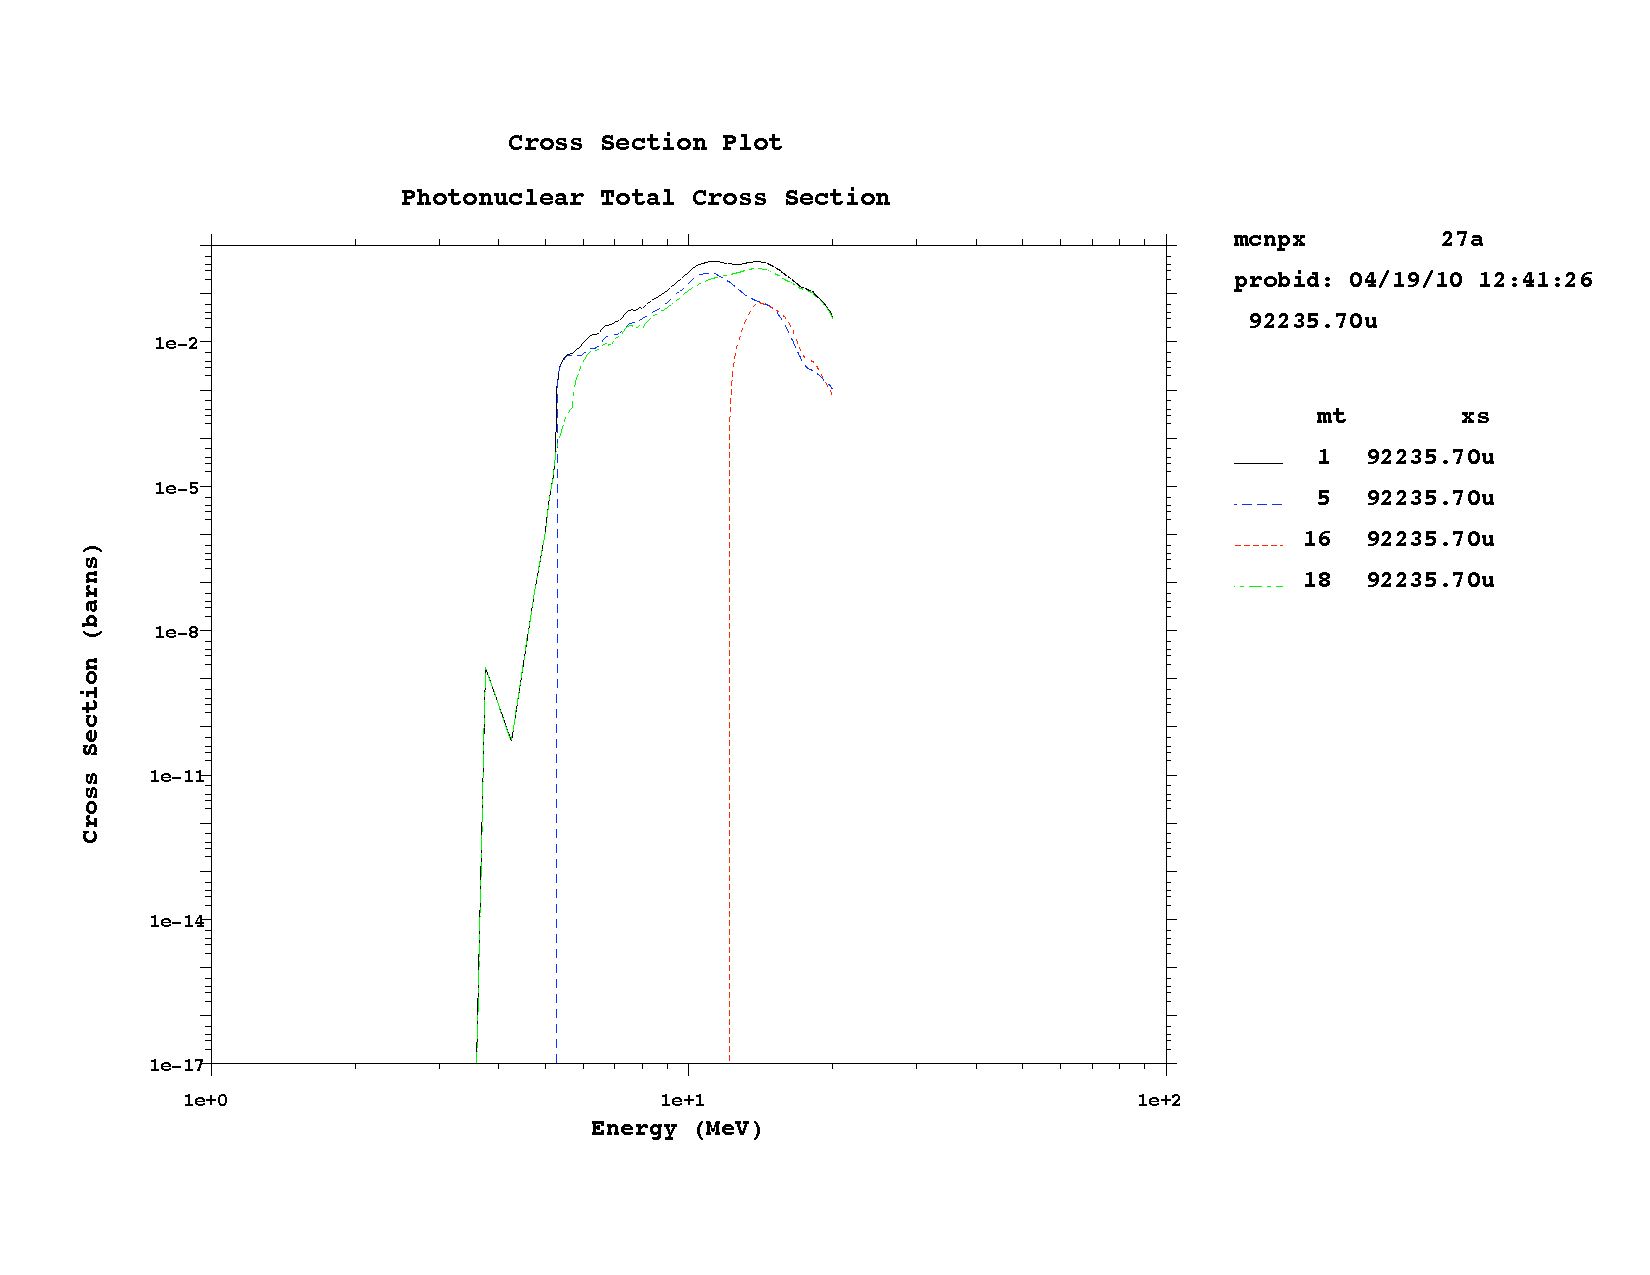
\includegraphics[scale=0.6, angle=0]{eps/92235_photonuclear.pdf}
\end{center}
\caption{Photonuclear cross-sections for $^{235}$U (taken from 92235.70u). Black curve is total, red curve is ($\gamma$,2n), green curve is photofission, blue is all other photonuclear reactions.} 
\label{fig:U-235 photonuclear cross-section}
\end{figure}

The {\tt MCNPX} input deck that describes this example is given below:
{\scriptsize
\begin{verbatim}
12 MeV x-rays into U-235
1 1 -19.0 -1 imp:n=1
2 0 1 imp:n=0

1 so 1.0

mode n p
m1 92235 1 pnlib=.70u
PHYS:P j 1 j -1 2j 1 $ 0=ACE,1=LLNL
sdef par=p erg=12
LCA 7j -2
nps 1000000
f1:n 1
e1 1e-6 199log 12
f11:p 1
e11 1e-3 199log 12
ft11 tag 3
fu11 -1 0.00004 92000.00003 92235.00005 92000.00005 92235.00018 1e10
\end{verbatim}}

To switch from the default ACE {\tt MCNPX} model to the LLNL photofission library, the $7^{th}$ entry of the PHYS:P is set to 1 in the input deck. Note that the $4^{th}$ entry of the PHYS:P card is set to -1 to turn on analog photonuclear particle production. We are interested here in the spectrum of prompt photofission gamma-rays emitted by $^{235}$U. Figure~\ref{fig:energy spectrum of the photofission gamma-rays from a 12 MeV gamma-ray beam impinging on 235U} shows the energy distribution of the photofission gamma-rays for different {\tt MCNPX} settings.

\begin{figure}[ht]
\begin{center}
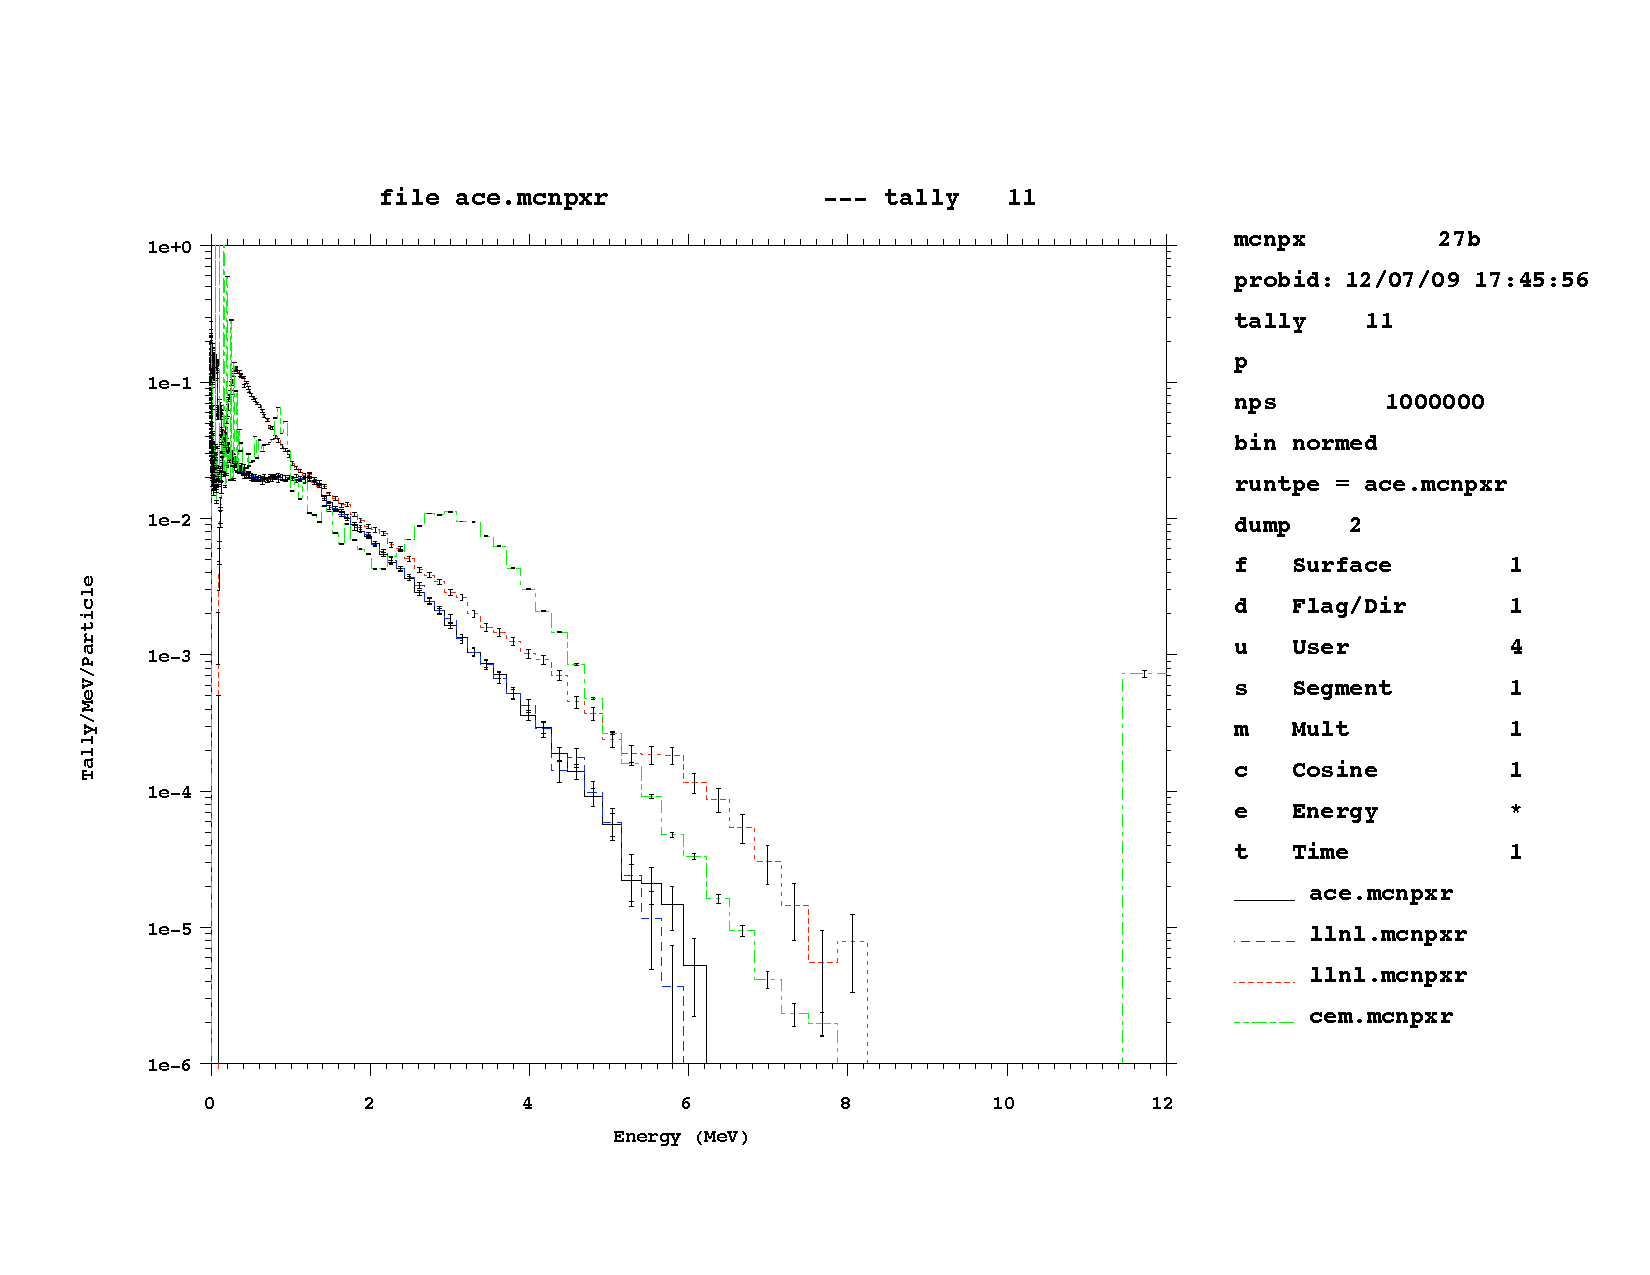
\includegraphics[width=\textwidth]{eps/PhotofissionGammaSpectrum.pdf}
\end{center}
\caption{Energy spectrum of the photofission gamma-rays from a 12 MeV gamma-ray beam impinging on $^{235}$U. The black, blue \& red, and green curves were generated by {\tt MCNPX} simulations with the ACE, LLNL, and CEM models, respectively.}
\label{fig:energy spectrum of the photofission gamma-rays from a 12 MeV gamma-ray
beam impinging on 235U}
\end{figure}

The black curve was generated from a  simulation with the ACE model, it shows the spectrum of all gamma-rays produced 
by photonuclear reactions with the ACE model. The default {\tt MCNPX} ACE model produces prompt photofission 
neutrons but does not produce any prompt photofission gamma-rays, because there is no such data available in the 
photonuclear data libraries ENDF/B-VII. 

The blue and red curves were generated from a simulation where the LLNL photofission library was turned on. The red curve is the spectrum of gamma-rays produced by photofission, while the blue one corresponds to gamma-rays produced by all other photonuclear reactions.

Finally, a last simulation was performed with the much slower CEM model, and the green curve shows the gamma-ray spectrum of all photonuclear reactions with this model.

\subsection{{\tt MCNP6}}\label{sec:mcnp}

Version 1.8 of this library was incorporated into the public release of {\tt MCNP6}. Version 2.0 is now incorporated into {\tt MCNP6.2}. For users with access to the {\tt MCNP6} source code, upcoming versions of this library can be compiled and linked, see \texttt{src/Recipe\_mcnpx.txt}. Consult the file \texttt{Release\_notes.txt} for comments regarding version compatibility.
Currently {\tt MCNP6} provide data cards to activate the fission library (individually for spontaneous, neutron-induced, and photon-induced fission), but do not yet permit changing any of the physics options of the library. 

In {\tt MCNP6.2}, treatment of fission photons is slightly different from what it is in {\tt MCNPX2.7.0}. See {\tt MCNP6.2} User Manual for details.

\subsubsection*{Neutron-induced and spontaneous fission model}

To enable sampling of neutrons and gamma-rays using this fission library set the {\tt METHOD} keyword on the FMULT card
to 5:
\begin{verbatim}
	FMULT zaid METHOD=5
\end{verbatim}
The LLNL fission model is the only way in {\tt MCNP6.2} to produce prompt fission photons. When the LLNL fission multiplicity package is selected (METHOD=5), both the prompt neutrons and the prompt fission photons are fully correlated with the fission event and have multiplicities.

Furthermore, when spontaneous fission reactions are activated, i.e.,
\begin{verbatim}
	SDEF PAR=SF
\end{verbatim}
the LLNL model is the only {\tt MCNP6} method emitting prompt photons for spontaneous fissions. In the case of spontaneous fissions, only the isotopes listed in Section~\ref{Limitations of the fission library} have data in the fission library. For other spontaneous fission isotopes, no neutrons, nor gamma-rays are emitted. Spontaneous fission photons are neglected in the {\tt MCNP6} default FMULT spontaneous fission source.

Delayed fission gammas are independent of the fission model and are controlled by the ACT card.

\subsubsection*{Photon-induced fission model}

When METHOD 5 is selected on the FMULT card and photofission is also turned on (ISPN$\ne$0 and FISM=1 on the PHYS:P card):
\begin{verbatim}
        PHYS:P 3J -1 2J 1
\end{verbatim}
prompt photofission gammas are generated with appropriate photofission neutron correlation and multiplicities. The same remarks as the ones in Sec.~\ref{sec:mcnpx} for the photon-induced fission model, apply here as well.


% !TEX root =  fission.tex
\pagebreak
\subsection{{\tt Geant4}}\label{sec:geant4}

Version 1.2 of this library has been available in the public release of Geant4 since version 4.9.0. 
Geant4.9.6 and later require version 1.9 or later of this library. Version 2.0 of the LLNL Fission Library has been tested with Geant4.10.02 as an external library that overrides the built-in fission library. It is available at \httpnuclear  . 
% To use the built-in version there is no need to download or compile the fission library itself and the standard Geant4 makefile is sufficient. 
An example of building a Geant4 executable and activating the fission library is given in the \texttt{geant} directory 
in the fission library source code distribution. This directory also includes an example and explicit instructions for overriding the built-in fission library with the latest version.

\subsection*{Limitations}

The neutron-induced fission data available in G4NDL4.5 is limited. At the time of this writing, there are only data files for  isotopes of radium, actinium, thorium, protactinium and uranium. The origin of the data has not been investigated. For other isotopes, induced fission will not emit any particles. This fission library does not have any spontaneous fission data for isotopes other than the ones listed in section~\ref{Limitations of the fission library}.
Photofission has not been implemented in {\tt Geant4}.

\subsection*{Execution}

The environment variable \textit{NeutronHPCrossSections} must point to the G4NDL directory, where the induced fission cross-sections and data are located.

\subsection*{Description of the C++ classes}


For neutron induced fission, this model is intended to be used with
the low energy neutron interaction data libraries with class
\textit{G4Fisslib} specified in the physics list as the
\textit{G4HadronFissionProccess} instead of class
\textit{G4NeutronHPFission}.\notgeant{
Here is an example code snippet for registering this model in the physics 
list: \input{snippet}}
The constructor of \textit{G4FissLib}
does two things. First it reads the necessary fission cross-section
data in the file located in the directory specified by the environment
variable \textit{NeutronHPCrossSections}. It does this by initializing
one object of class \textit{G4NeutronHPChannel} per isotope present in
the geometry. Second, it registers an instance of
\textit{G4FissionLibrary} for each isotope as the model for that
reaction/channel. When Geant4 tracks a neutron to a reaction site and
the fission library process is selected among all other process for
neutron reactions, the method \textit{G4FissLib::ApplyYourself} is
called, and one of the fissionable isotopes present at the reaction
site is selected. This method in turn calls
\textit{G4NeutronHPChannel::ApplyYourself} which calls
\textit{G4FissionLibrary::ApplyYourself}, where the induced neutrons
and gamma-rays are emitted by sampling the fission library.

For spontaneous fission the user must provide classes {\it
PrimaryGeneratorAction}, {\it MultipleSource}, {\it
MultipleSourceMessenger}, {\it SingleSource}, {\it SponFissIsotope} to
generate spontaneous fission neutrons and gammas. Examples of these
classes can be downloaded from \httpnuclear. Spontaneous fissions are
generated in the {\it PrimaryGeneratorAction} class.
The spontaneous fission
source needs to be described in terms of geometry, isotopic
composition and fission strength. Once this information is given, the
constructor creates as many spontaneous fission isotopes of class {\it
SponFissIsotope} as specified, and adds them to the source of class
{\it MultipleSource}. When Geant needs to generate particles, it calls
the method {\it PrimaryGeneratorAction::GeneratePrimaries}, which
first sets the time of the next fission based on the fission rates
entered in the constructor, and then calls the method {\it
MultipleSource::GeneratePrimaryVertex} which determines which one of
the spontaneous fission isotopes will fission. This method in turn
calls the method {\it SponFissIsotope::GeneratePrimaryVertex} for the
chosen isotope. It is in this method that the neutrons and photons
sampled from the fission library are added to the stack of secondary
particles.  Sources other than spontaneous fission isotopes can be
added to the source of class {\it MultipleSource}. For instance, a
background term emitting a large number of background gamma-rays can
be added, as long as it derives from the class {\it SingleSource}. The
intensity of that source would be set the same way as for the
spontaneous fission isotope sources.



%\pagebreak
\subsection{COG}
This physics module has been submitted to the COG development team
and will appear in a future release.  The fission library libFission.a
can be sampled for induced fissions in COG using the \textit{FISSLIB}
keyword in the MIX block of the input deck. This is not the
default. The \textit{NUOPTION} can not be used concurrently, it is not
compatible with \textit{FISSLIB}.

COG is similar to MCNPX in that it emits a number of gamma-rays
at each neutron collision site, and this number is independent
on the reaction type. The keyword \textit{NOGAMPRO} can be used
to completely turn off this gamma-ray production.

Spontaneous fissions are implemented using a COG user source.
A sample user source {\tt spfiss.F} is available in the COG distribution 
subdirectory {\tt usrsor}. Compiling a COG user source is easy:
\begin{verbatim}
	make -f COGUserlib.make in=spfiss.F
\end{verbatim}
Using the right compiler at compile time is important, and if this
becomes an issue, a COG developer should be contacted. It is also 
important to use a COG version that is compatible with user
sources and user detectors. Not all COG versions work with
user sources/detectors. Photofission has not been implemented in
COG.

An example of input deck using the {\tt spfiss.F} spontaneous
fission source is located in the {\tt usrsor} directory. The important
lines related to the user source are in the SOURCE block:

{ \small
\begin{verbatim}
SOURCE
NPART = 5e4  $ NPART is the sum of spontaneous fission neutrons and photons
$ 
$ The source below is for a HEU shell (93% enriched in U-235).
$ We neglect here the spontaneous fissions in U-235. The fission rate 
$ for 350 g of U-238 is 350[g]*1.36*10E-2[n/g/s] = 4.76 n/s. With
$ spontaneous nubar equal to 2.01, we have 
$  4.76[n/s]/2.01[n/fission] = 2.368 fissions/sec
$      name    isotope  strength  xcenter  ycenter  zcenter  Rin  Rout  FissRate
$              (1)      (2)       (3)      (4)      (5)      (6)  (7)   (8)
USRSOR spfiss  92238    1.        0.       0.       0.       1.   3.96  2.368
$
\end{verbatim}
}
NPART is the sum of all source particles, that is both spontaneous
fission neutrons and gamma-rays. The line USRSOR has several arguments:
The argument under {\tt name} specify the FORTRAN subroutine to be used a 
the spontaneous fission source: {\tt spfiss}. The first numeric argument is 
the isotope in the form ZA, followed by the source strength (not relevant
in this case), the center of the shell (x, y, z), the inner and outer
radii and the fission rate in fissions/second. Note the units of the
fission rate, fissions/second and not neutrons/second.


% !TEX root =  fission.tex
\pagebreak
\subsection{Fission library interface}\label{sec:api}

The interface to the fission library consists of 27 C functions, each of which will be described below. For examples of creating a stand-alone executable with the programmer's interface, consult the directory \texttt{regr} in the software release.

\subsection*{void genspfissevt\_(int *isotope, double *time)}
This function is called to trigger a spontaneous fission. Multiple neutrons and gamma-rays are generated and stored in a stack along with their energies, directions and emission times. The arguments of this function are

\begin{tabbing}
\indent isotope: \=entered in the form ZA (e.g. 94239 for $^{239}$Pu) \\
\indent time: \> the time of the spontaneous fission \\
\end{tabbing}

The generated neutrons and gamma-rays, along with their properties will be lost upon the next call to genspfissevt\_(),
genfissevt\_() or genphotofissevt\_(). Therefore, they must be retrieved immediately by the caller using the appropriate 
functions described below.

\subsection*{void genfissevtdir\_(int *isotope, double *time, double *nubar, double *eng, double *ndir)}
This function is called to trigger a neutron-induced fission. In addition to the arguments above, the fission inducing neutron
is characterized by:

\begin{tabbing}
\indent nubar: \= user-specified average number of neutrons emitted per fission (e.g. as tabulated in the \\ 
\> cross-section libraries used by the particle transport code) \\
\indent eng: \> energy of the neutron inducing fission \\
\indent ndir: \> normalized incident neutron direction, array with three elements (u,v,w) \\
\end{tabbing}

Either the average number $\bar{\nu}$ of neutrons emitted per fission or the energy \textit{eng} of the fission inducing 
neutron will be used to determine the number of neutrons sampled, see function setnudist\_ below. The number 
of gamma-rays sampled only depends on $\bar{\nu}$. Similarly to genspfissevt\_(), the generated neutrons and gamma-rays are lost upon subsequent calls to genspfissevt\_(), genfissevt\_() or genphotofissevt\_(). The direction $ndir$ of the incident neutron is only used by the {\tt FREYA} model.

\subsection*{void genfissevt\_(int *isotope, double *time, double *nubar, double *eng)}
Same as call to {\bf genfissevtdir\_()} but {\tt FREYA} samples the incident neutron direction randomly.

\subsection*{void genphotofissevt\_(int *isotope, double *time, double *nubar, double *eng)}
This function is called to trigger a photon-induced fission. In addition to the arguments specified in genfissevt\_, the 
fission inducing neutron is characterized by:

\begin{tabbing}
\indent nubar: \= user-specified average number of neutrons emitted per photofission (e.g. as tabulated in the \\ 
\> photonuclear cross-section libraries used by the particle transport code) \\
\indent eng: \> energy of the photon inducing fission \\
\end{tabbing}

Either the average number $\bar{\nu}$ of neutrons emitted per photofission or the energy \textit{eng} of the fission inducing 
photon will be used to determine the number of neutrons sampled, see function setnudist\_ below. The number of gamma-rays sampled only depends on $\bar{\nu}$. Similarly to genspfissevt\_(), the generated neutrons and gamma-rays are lost upon subsequent calls to genspfissevt\_(), genfissevt\_() or genphotofissevt\_().

\subsection*{int getnnu\_() and int getpnu\_()}

These functions return the numbers of fission neutrons and gamma-rays emitted in the fission reaction, or -1 if no number could be sampled in the fission library due to lack of data. The reader is referred to the physics reference manual to find the list of isotopes for which sampling will return positive numbers.

\subsection*{double getneng\_(int *index) and 
double getpeng\_(int *index) \newline
double getnvel\_(int *index) and 
double getpvel\_(int *index)}

These functions return the energies and velocities of the neutrons/gamma-rays.

\subsection*{double getndircosu\_(int *index), double getndircosv\_(int *index), \newline double getndircosw\_(int *index) \newline \newline
double getpdircosu\_(int *index), double getpdircosv\_(int *index), \newline double getpdircosw\_(int *index)}

These 2 families of functions return the direction cosines of the velocity vector on the x, y and z axes for the fission 
neutrons and gamma-rays.

\subsection*{double getnage\_(int *index) and double 
getpage\_(int *index)}

This functions returns the age of the fission neutron/gamma-ray, or -1 if index is out of range. The age returned might be 
different from the time specified in genfissevt\_(), genspfissevt\_() and genphotofissevt\_() for delayed neutrons and gamma-rays, see function setdelay\_() below. Currently, delayed fission neutrons/gamma-rays are not implemented, so all fission products 
are emitted promptly.

\subsection*{void setdelay\_(int *delay)}~\label{setdelay}

This function is called to enable delayed neutrons and gamma-rays. The argument \textit{delay} is set to 

\begin{tabbing}
\indent0 (default) \= for strictly prompt neutrons and photons \\
\indent1 (n/a) \> for prompt neutrons, prompt and delayed photons \\
\indent2 (n/a) \> for prompt and delayed neutrons, prompt photons \\
\indent3 (n/a) \> for prompt and delayed neutrons, prompt and delayed photons \\
\end{tabbing}

Delayed neutrons and gamma-rays have not yet been implemented in the fission library. This setting has presently no effect on the age sampling. All neutrons and photons are currently emitted promptly (delay=0).

\subsection*{void setcorrel\_(int *correlation)}\label{setcorrel}

This function is called to set the type of neutron/gamma-ray correlation.  The argument \textit{correlation} is set to

\begin{tabbing}
\indent 0 (default) \= for no correlation between neutrons and photons \\
\indent 1 \> \parbox[t]{5.5in}{total fission neutron energy and total fission gamma-ray energy are sampled from normal distributions of means given in Beck et al.~\cite{Beck 2007}. No correlation between the number of neutrons and the number of gamma-rays} \\
\indent 2 \> \parbox[t]{5.5in}{total fission neutron energy and total fission gamma-ray energy are sampled from normal distributions of means given in Vogt~\cite{Vogt 2008}. No correlation between the number of neutrons and the number of gamma-rays} \\
\indent 3 \> \parbox[t]{5.5in}{number and energy correlation between neutrons and photons provided by {\tt FREYA} whenever available.} \\
\end{tabbing}

% !TEX root =  fission.tex
\subsection*{void setnudist\_(int *nudist)
\label{setnudist}}

This selects the data to be sampled for the neutron number distributions for neutron-induced fission. If there is no data
available, then in all cases the Terrell approximation is used. The argument \textit{nudist} can take 3 values:

\begin{tabbing}

\indent 0 \hspace*{.55in} \= \parbox[t]{5.5in}{ Use the fit to the Zucker and Holden tabulated P$_\nu$ distributions as a function of energy for $^{235}$U, $^{238}$U and $^{239}$Pu.}\\

\indent 1 \> \parbox[t]{5.5in}{Use fits to the Zucker and Holden tabulated P$_\nu$  distribution as a function of energy for $^{238}$U and  $^{239}$Pu, and a fit to the Zucker and Holden data as well as the Gwin, Spencer and Ingle data (at thermal 
 energies) as a function of energy for $^{235}$U.}\\

\indent 2 \> \parbox[t]{5.5in}{Use the fit to the Zucker and Holden tabulated P$_\nu$ distributions as a function of $\bar{\nu}$. The $^{238}$U fit is used for the $^{232}$U, $^{234}$U, $^{236}$U and $^{238}$U isotopes, the $^{235}$U fit for $^{233}$U 
and $^{235}$U, the $^{239}$Pu fit for $^{239}$Pu and $^{241}$Pu.}\\

\indent 3 (default) \> \parbox[t]{5.5in}{Use the discrete Zucker and Holden tabulated P$_\nu$ distributions and corresponding $\bar{\nu}$s. Sampling based on the incident neutron $\bar{\nu}$. The $^{238}$U data tables are used for the $^{232}$U, $^{234}$U, $^{236}$U  and $^{238}$U isotopes, the $^{235}$U data for $^{233}$U and $^{235}$U, the $^{239}$Pu data for $^{239}$Pu and $^{241}$Pu.}

\end{tabbing}

\subsection*{void setcf252\_(int *ndist, int *neng)}

This function is specific to the spontaneous fission of $^{252}$Cf. It selects the data to be sampled for the neutron number and energy distributions and takes the following arguments:

\begin{tabbing}
\indent ndist: \= Sample the number of neutrons \\
\indent \> 0 (default) \= 
from the tabulated data measured by Spencer \\
\indent \> 1 \> from 
Boldeman's data \\
\\
\indent neng: Sample the spontaneous fission 
neutron energy \\
\indent \> 0 (default)\> from Mannhart corrected  Maxwellian spectrum \\
\indent \> 1 \> from Madland-Nix theoretical spectrum \\
\indent \> 2 \> from the Froehner Watt spectrum \\
\end{tabbing}

\subsection*{void getfreya\_errors\_(int *length, char *error)}
When called, this function returns potential errors that could have occurred in {\tt FREYA}; for instance if the data required by {\tt FREYA} cannot be found. It takes the following arguments:
\begin{tabbing}
\indent length: \= length of error message \\
\indent error: \> pointer to an allocated array of characters devoted to the error message \\
\end{tabbing}
When returning, the length of the error message will be 1 is no error occurred. It will be greater than 1 otherwise.

\subsection*{void setfreyadatapath\_(char *path)}
This function is called to set the path to the directory where the data required by {\tt FREYA} is located. It takes the following argument:
\begin{tabbing}
\indent path: \= character string containing the path to the directory containing the data required by {\tt FREYA}. \\
\end{tabbing}



\subsection*{void setrngf\_(float (*funcptr) (void)) and void setrngd\_(double (*funcptr) (void))}

This function sets the random number generator to the user-defined
one specified in the argument. If either setrngf\_() or setrngd\_() are
not specified, the default system call srand48() is used. The 
arguments are random number generator functions that returns 
variables of type float and double respectively.

 \clearpage

\addcontentsline{toc}{section}{References}

\begin{thebibliography}{99}
% !TEX root =  fission.tex

\bibitem{Verbeke 2016} J.M. Verbeke, J. Randrup, R. Vogt, ``Fission Reaction Event Yield Algorithm FREYA 2.0 User Manual,'' LLNL-TR-XXXXXX , Lawrence Livermore National Laboratory, Livermore, California (2016).

\bibitem{Terrell 1957} J. Terrell, "Distributions of Fission Neutron
Numbers", \textit{Phys. Rev.} \textbf{108}, 783 (1957).

\bibitem{Zucker and Holden 1986} M.S. Zucker, N.E. Holden, "Energy
Dependence of Neutron Multiplicity P$_{\nu}$ in Fast-Neutron-Induced
Fission for $^{235,238}U$ and $^{239}Pu$," BNL-38491 (1986).

\bibitem{Cullen 2006} D.E. Cullen, "Sampling the Number of Neutrons
Emitted per Fission," UCRL-TR-222526, Lawrence Livermore National
Laboratory (2006).  

\bibitem{Gwin 1984} R. Gwin, R.R. Spencer,
R.W. Ingle, "Measurements of the Energy Dependence of Prompt Neutron
Emission from $^{233}U$, $^{235}U$, $^{239}Pu$, and $^{241}Pu$ for
$E_n=0.005$ to 10 eV Relative to Emission from Spontaneous Fission of
$^{252}$Cf," \textit{Nucl. Sci. Eng.}, \textbf{87}, 381 (1984).

\bibitem{Valentine 1996} T.E. Valentine, J.T. Mihalczo, "MCNP-DSP: A
Neutron and Gamma Ray Monte Carlo Calculation of Source-Driven
Noise-Measured Parameters ," \textit{Ann. of Nucl. Eng.}, \textbf{23},
16, p. 1271 (1996).

\bibitem{Valentine 2000} T.E. Valentine, "MCNP-DSP Users Manual,"
ORNL/TM-13334, R2, Oak Ridge National Laboratory (2000).

\bibitem{Frehaut 1988} J. Frehaut, "Neutron Multiplicity Distribution
in Fast Neutron-Induced Fission," \textit{Proc. of IAEA Consultant's
Meeting on Physics of Neutron Emission in Fission,}, Mito, Japan
(1988).  

\bibitem{Holden and Zucker BNL} N.E. Holden,
M.S. Zucker, "A Reevaluation of the Average Prompt Neutron Emission
Multiplicity ($\bar{\nu}$) Values from Fission of Uranium and
Transuranium Nuclides," BNL-NCS-35513, Brookhaven National
Laboratory).  

\bibitem{Santi 2005} P. Santi, D.H. Beddingfield, D.R. Mayo, "Revised
prompt neutron emission multiplicity distributions for $^{236,238}$Pu,"
 \textit{Nucl. Phys. A} \textbf{756}, 325-332 (2005).

\bibitem{BNL-36467} BNL-36467.

\bibitem{Dakavoski 1973} Dakavoski, \textit{Sov.Atom.Erg.} \textbf{17},
360, BNL-36467, (1973).

\bibitem{Hoffman 1980} Hoffman, \textit{Phys.Rev.C.} \textbf{21},
637, BNL-36467, (1980).

\bibitem{Lazarev 1974} Lazarev, \textit{Phys.Lett.} \textbf{52B},
321, BNL-36467, (1974).

\bibitem{Spencer 1982} R.R. Spencer, R. Gwin, R.W. Ingle, "A
measurement of the Average Number of Prompt Neutrons from Spontaneous
Fission of Californium-252," \textit{Nucl. Sci. Eng.} \textbf{80}, 603
(1982).  

\bibitem{Boldeman 1985} J.W. Boldeman, M.G. Hines, "Prompt
Neutron Emission Probabilities Following Spontaneous and Thermal
Neutron Fission," \textit{Nucl. Sci. Eng.}, \textbf{91}, 114 (1985).

\bibitem{Ensslin 1998} N. Ensslin, W.C. Harker, M.S. Krick,
D.G. Langner, M.M. Pickrell, J.E. Stewart, "Application Guide to
Neutron Multiplicity Counting," LA-13422-M, Los Alamos National
Laboratory (1998).  

\bibitem{ENDL 1975} R.J. Howerton, et al, "The LLL
Evaluated Nuclear Data Library (ENDL): Evaluation Techniques, Reaction
Index, and Description of Individual Evaluations," UCRL-50400, V. 15,
Part A, Lawrence Livermore National Laboratory (1975).

\bibitem{TART 2003} D.E. Cullen, "TART 2002: A Couple
Neutron-Photon 3-D, Combinatorial Geometry, Time Dependent Monte-Carlo
Transport Code," UCRL-ID-126455, Rev. 4, Lawrence Livermore National
Laboratory (2003).  

\bibitem{Cullen 2004} D.E. Cullen, "Sampling ENDL Watt Fission
Spectra," UCRL-TR-203251, Lawrence Livermore National Laboratory
(2004).  

\bibitem{Everett 1983} C.J. Everett, E.D. Cashwell, "A Third
Monte Carlo Sampler," LA-9721-MS, Los Alamos National Laboratory
(1983).  


\bibitem{Mannhart 1987} W. Mannhart, "Evaluation
of the Cf-252 Fission Neutron Spectrum Between 0 MeV and 20 MeV,"
\textit{Proc. Advisory Group Mtg. Neutron Sources}, Leningrad, USSR,
1986 (IAEA-TECDOC-410), Vienna (1987).  

\bibitem{Madland 1984}
D.G. Madland, J.R. Nix, "Prompt Fission Neutron Spectra and Average
Prompt Neutron Multiplicities,"NEANDC Specialist's Meeting on Yields
and Decay Data of Fission Products, Brookhaven National Laboratory,
BNL 51778 (1984).  

\bibitem{Froehner 1990} F.H. Fr\"{o}hner,
"Evaluation of $^{252}$Cf Prompt Fission Neutron Data from 0 to 20 MeV
by Watt Spectrum Fit," \textit{Nucl. Sci. Eng.} \textbf{106}, 345
(1990).  

\bibitem{Beck 2007} B. Beck, D.A. Brown, F. Daffin, J. Hedstrom, 
R. Vogt, "Implementation of Energy-Dependent Q Values for Fission,"
UCRL-TR-234617, Lawrence Livermore National Laboratory (2007).  

\bibitem{Madland 1982} D. Madland, J.R. Nix, \textit{Nucl. Sci. and
Eng.} \textbf{81}, p.213 (1982).

\bibitem{Vogt 2008} R. Vogt, "Energy-Dependent Fission Q Values 
Generalized for All Actinides," LLNL-TR-407620, Lawrence Livermore 
National Laboratory (2008).  

\bibitem{Brunson 1982} G.S. Brunson, Jr., "Multiplicity and
Correlated Energy of Gamma Rays Emitted in the Spontaneous Fission of
Californium-252," Ph.D. Thesis, University of Utah (1982).

\bibitem{Valentine 2001} T.E. Valentine, "Evaluation of Prompt Fission
Gamma Rays for Use in Simulating Nuclear Safeguard Measurements,"
\textit{Ann. Nucl. Eng.}, \textbf{28}, 191 (2001).  

\bibitem{Wagemans
1991} C. Wagemans, "The Nuclear Fission Process," \textit{CRC Press,
Inc.,} Boca Raton, Florida (1991).  

\bibitem{Maienschein 1958}
F.C. Maienschein, R.W. Peelle, T.A. Love, \textit{Neutron
Phys. Ann. Prog. Rep. for Sept. 1, 1958}, ORNL-2609, Oak Ridge
National Laboratory (1958).  

\bibitem{Goldstein 1959} "Fundamental
Aspects of Reactor Shielding," Addison-Wesley Publishing Company,
Inc. Reading, Massachussetts (1959).

\bibitem{Oblozinsky 1998} "Summary Report of the $2^{nd}$ Research Coordination 
Meeting on Compilation and Evaluation of Photonuclear Data for 
Applications," International Atomic Energy Agency Report INDC(NDS)-384, 
Vienna, Austria (1998).

%\bibitem{McLane 1997} V. McLane, C.L. Dunford and P.F. Rose, "ENDF-102 Data 
%Formats and Procedures for the Evaluated Nuclear Data File ENDF-6," Report 
%BNL-NCS-44945 Rev. 2/97, Brookhaven National Laboratory, Upton, New York (1997).

\bibitem{Chadwick 1999} M.B. Chadwick et al., "Cross-Section Evaluations to 
150 MeV for Accelerator-Driven Systems and Implementation in MCNPX," 
\textit{Nuclear Science and Engineering,} \textbf{131,} pp. 293-328 (1999).

\bibitem{IAEAphoto} P. Oblo{\v z}insk{\' y}, ed. ``Handbook of photonuclear data for applications: Cross sections and spectra,'' International Atomic Energy Association report IAEA-TECDOC-1178, Vienna, Austria (2000).

\bibitem{ENDFB7} M.B. Chadwick, P. Oblo{\v z}insk{\' y}, M. Herman, N.M. Greene, R.D. McKnight, D.L. Smith, P.G. Young, R.E. MacFarlane, G.M. Hale, S.C. Frankle, A.C. Kahler, T. Kawano, R.C. Little, D.G. Madland, P. Moller, R.D. Mosteller, P.R. Page, P. Talou, H. Trellue, M.C. White, W.B. Wilson, R. Arcilla, C.L.Dunford, S.F. Mughabghab, B. Pritychenko, D. Rochman, A.A. Sonzogni, C.R. Lubitz, T.H. Trumbull, J.P. Weinman, D.A. Brown, D.E. Cullen, D.P. Heinrichs, D.P. McNabb, H. Derrien,
M.E. Dunn, N.M. Larson, L.C. Leal, A.D. Carlson, R.C. Block, J.B. Briggs, E.T. Cheng, H.C. Huria, M.L. Zerkle, K.S. Kozier, A. Courcelle, V. Pronyaev and S.C. van der Marck, ``{ENDF/B-VII.0}: Next Generation Evaluated Nuclear Data Library for Nuclear Science and Technology,''
{\em Nuclear Data Sheets}, {\textbf 107}, pp.~2931-3060 (2006), ISSN 0090-3752, DOI: 10.1016/j.nds.2006.11.001,
(\url{http://www.sciencedirect.com/science/article/B6WNV-4MGDW8W-1/2/5040b3d5640d1c334634e9f83c754893}).

\bibitem{Firestone 1996} R.B. Firestone, V.S. Shirley, C.M. Baglin, S.Y.F. Chu, J. Zipkin, "The 8th edition of the Table of Isotopes," Wiley \& Sons, Inc. (1996).

\bibitem{Wapstra 2003} A.H. Wapstra, G. Audi, C. Thibault, "The AME2003 atomic mass evaluation (I). Evaluation of input data, adjustment procedures," {\em Nuclear physics} {\textbf A729,} 129 (2003).

\bibitem{Audi 2003} G. Audi, A.H. Wapstra, C. Thibault, "The AME2003 atomic mass evaluation (II). Tables, graphs, and references," {\em Nuclear physics} {\textbf A729,} 337 (2003).

\bibitem{MCNPX} "MCNPX Version 2.5.0 User's Manual", LA-CP-05-0369, Los Alamos National Laboratory (2005).

\bibitem{Geant1} 
S. Agostinelli, {\it et al.}
``Geant4 a simulation toolkit''
Nucl.\ Instrum.\ Meth.\ A {\bf 506}, 250-303 (2003).

\bibitem{Geant2} 
J. Allison et al., {\it et al.}
``Geant4 developments and applications''
IEEE Trans. Nucl. Sci. {\bf 53}, 270-278 (2006). 
\end{thebibliography}

\end{document}
